% -*- Mode:TeX -*-

%% IMPORTANT: The official thesis specifications are available at:
%%            http://libraries.mit.edu/archives/thesis-specs/
%%
%%            Please verify your thesis' formatting and copyright
%%            assignment before submission.  If you notice any
%%            discrepancies between these templates and the 
%%            MIT Libraries' specs, please let us know
%%            by e-mailing thesis@mit.edu

%% The documentclass options along with the pagestyle can be used to generate
%% a technical report, a draft copy, or a regular thesis.  You may need to
%% re-specify the pagestyle after you \include  cover.tex.  For more
%% information, see the first few lines of mitthesis.cls. 

%\documentclass[12pt,vi,twoside]{mitthesis}
%%
%%  If you want your thesis copyright to you instead of MIT, use the
%%  ``vi'' option, as above.
%%
%\documentclass[12pt,twoside,leftblank]{mitthesis}
%%
%% If you want blank pages before new chapters to be labelled ``This
%% Page Intentionally Left Blank'', use the ``leftblank'' option, as
%% above. 

\documentclass[10.5pt,twoside]{mitthesis}
\usepackage{lgrind, afterpage}
\usepackage{fancyhdr}
\usepackage[sc]{mathpazo}
%% These have been added at the request of the MIT Libraries, because
%% some PDF conversions mess up the ligatures.  -LB, 1/22/2014
\usepackage{cmap}
\usepackage{tabto}
\usepackage[T1]{fontenc}
%\usepackage[english]{babel}
%\usepackage[spanish,es-tabla]{babel}
\usepackage[spanish,es-tabla,es-nosectiondot]{babel} % spanish
\usepackage{graphicx}
\usepackage{appendix}
\usepackage{eurosym}
\usepackage{comment}
\usepackage{subcaption}
\usepackage{epigraph}
\usepackage[export]{adjustbox}
\usepackage{amsmath} % equations
\usepackage{mathtools}
\usepackage{algorithm}
\usepackage{algorithmicx}
\usepackage{algpseudocode}
\usepackage[textfont=it]{caption}
\usepackage[hidelinks]{hyperref}
\usepackage[acronym]{glossaries}
\usepackage[svgnames]{xcolor}
\usepackage{array,booktabs,makecell,rotating,ragged2e} % nice tables
\usepackage{pifont}	% check
\usepackage{listings} % linux commands
\usepackage[utf8]{inputenc}
%\usepackage[demo]{graphicx}
\makeglossaries
\pagestyle{plain}

\definecolor{mycolor}{gray}{0.15}  % Outer background color of 

  \makeglossaries
  
% Traceability matrix
\renewcommand*\theadfont{\bfseries}
\settowidth\rotheadsize{\theadfont Infrastructure}
\renewcommand\theadgape{}
\renewcommand\theadalign{lc}
\renewcommand\rotheadgape{}

% START ALGORITHM

\captionsetup{compatibility=false}

\DeclareCaptionSubType*{algorithm}

\renewcommand\thesubalgorithm{\thetable\alph{subalgorithm}}

\DeclareCaptionLabelFormat{alglabel}{Algorithm~#2}

% END ALGORITHM

% epigraph
\setlength\epigraphwidth{8cm}
\setlength\epigraphrule{0pt}

\renewcommand{\listfigurename}{Lista de Figuras}
\renewcommand{\listtablename}{Lista de Tablas}
\renewcommand{\contentsname}{Lista de Contenidos}
\renewcommand{\figurename}{\textbf{\textit{Figura}}}
\renewcommand\bibname{Bibliografía}
\renewcommand{\lstlistingname}{Listado}

\renewcommand{\appendixname}{Anexos}
\renewcommand{\appendixtocname}{Anexos}
\renewcommand{\appendixpagename}{Anexos}



% pseudocode
\makeatletter
%\renewcommand{\ALG@name}{Pseudocode}
\makeatother
\renewcommand{\thealgorithm}{\thechapter.\arabic{algorithm}}% Algorithm # is <chapter>.<algorithm>
\makeatletter\@addtoreset{algorithm}{chapter}\makeatother
\makeatletter
\renewcommand{\ALG@beginalgorithmic}{\normalsize}
\makeatother

% xml
\usepackage{color}
\definecolor{gray}{rgb}{0.4,0.4,0.4}
\definecolor{darkblue}{rgb}{0.0,0.0,0.6}
\definecolor{cyan}{rgb}{0.0,0.6,0.6}

\lstset{
  basicstyle=\ttfamily,
  columns=fullflexible,
  showstringspaces=false,
  commentstyle=\color{gray}\upshape
}

\lstdefinelanguage{XML}
{
  morestring=[b]",
  morestring=[s]{>}{<},
  morecomment=[s]{<?}{?>},
  stringstyle=\color{black},
  identifierstyle=\color{darkblue},
  keywordstyle=\color{cyan},
  morekeywords={xmlns,version,type}% list your attributes here
}

\newcommand{\cmark}{\ding{51}}%
\newcommand{\xmark}{\ding{55}}%

\newcommand{\nref}[1]{(\ref{#1})}
\newcommand{\ivy}{{\sc Ivy\xspace}}

\lstset{
language=C++,
 frame=lines,
 basicstyle=\fontsize{7}{7}\ttfamily,
 captionpos=t,
 belowcaptionskip=\medskipamount,
commentstyle=\color{mygreen},
columns=fullflexible,
numbers=left,
numbersep=6pt,
numberstyle=\tiny\color{mygray},
keywordstyle=\color{mymagenta},
stringstyle=\color{myred},
breaklines=true,
escapeinside={<@}{@>},
emph={Farm,Pipeline,Accumulator,Filter,Map,Reduce,MapReduce,Stencil,DivideAndConquer}, 
emphstyle=\color{blue},
morekeywords={}
}

\newcommand{\rpr}{\textsc{Repara}\xspace}
\newcommand{\rph}{\textsc{RePhrase}\xspace}
\newcommand{\parboil}{\texttt{Parboil}\xspace}
\newcommand{\rodinia}{\texttt{Rodinia}\xspace}
\newcommand{\nas}{\texttt{NAS}\xspace}
\newcommand{\bioperf}{\texttt{BioPerf}\xspace}
\newcommand{\pipeline}{{\small\textsf{Pipeline}}\xspace}
\newcommand{\farm}{{\small\textsf{Farm}}\xspace}
\newcommand{\map}{{\small\textsf{Map}}\xspace}
\newcommand{\reduce}{{\small\textsf{Reduce}}\xspace}
\newcommand{\mapreduce}{{\small\textsf{MapReduce}}\xspace}
\newcommand{\stencil}{{\small\textsf{Stencil}}\xspace}
\newcommand{\filter}{{\small\textsf{Filter}}\xspace}
\newcommand{\accum}{{\small\textsf{Accumulator}}\xspace}
\newcommand{\dac}{{\small\textsf{Divide\&Conquer}}\xspace}
\newcommand{\grppi}{\textsc{GrPPI}\xspace}
\newcommand{\nfea}{\textsf{No-Factible}}%
\newcommand{\feas}{\textsf{Factible}}%
\newcommand{\usab}{\textsf{Usable-Reducible}}%
\newcommand{\irre}{\textsf{Irreducible}}%
\newcommand{\nfeas}{{\small\nfea}\xspace}%
\newcommand{\feasi}{{\small\feas}\xspace}%
\newcommand{\usabl}{{\small\usab}\xspace}%
\newcommand{\irred}{{\small\irre}\xspace}%
\newcommand{\nfeasm}{\xmark\ \tiny{(\nfea)}}%
\newcommand{\feasim}{\cmark\ \tiny{(\feas)}}%
\newcommand{\usablm}{\cmark\ \tiny{(\usab)}}%
\newcommand{\irredm}{\cmark\ \tiny{(\irre)}}%

\definecolor{mygray}{rgb}{0.4,0.4,0.4}
\definecolor{mygreen}{rgb}{0.2,0.7,0.2}
\definecolor{myorange}{rgb}{1.0,0.3,0}
\definecolor{mymagenta}{rgb}{0.6,0,0.6}
\definecolor{myred}{rgb}{0.8,0,0}

\usepackage{etoolbox}

% hyphenation
\hyphenation {ma-yo-res}


\makeatletter
\patchcmd{\epigraph}{\@epitext{#1}}{\itshape\@epitext{#1}}{}{}
\makeatother

\newcommand{\ra}[1]{\renewcommand{\arraystretch}{#1}}
\newcolumntype{L}[1]{>{\raggedright\let\newline\\\arraybackslash\hspace{0pt}}m{#1}}
\newcolumntype{C}[1]{>{\centering\let\newline\\\arraybackslash\hspace{0pt}}m{#1}}
\newcolumntype{R}[1]{>{\raggedleft\let\newline\\\arraybackslash\hspace{0pt}}m{#1}}

% encabezados
\lhead[\thepage]{\rightmark}
\chead[]{}
\rhead[Patrones de programación paralelos de alto nivel en arquitecturas de memoria distribuida\leftmark]{\thepage}
\renewcommand{\headrulewidth}{0.5pt}

\newcommand\blankpage{%
    \null
    \thispagestyle{empty}%
    \newpage}

% pie de pagina
\lfoot[]{}
\cfoot[]{}
\rfoot[]{}
\renewcommand{\footrulewidth}{0pt}

% primera pagina de un capitulo
\fancypagestyle{plain}{
\fancyhead[L]{}
\fancyhead[C]{}
\fancyhead[R]{}
\fancyfoot[L]{}
\fancyfoot[C]{\thepage}
\fancyfoot[R]{}
\renewcommand{\headrulewidth}{0pt}
\renewcommand{\footrulewidth}{0pt}
\cfoot{\thepage}
}

\pagestyle{fancy}

% Authors margins
\def\changemargin#1#2{\list{}{\rightmargin#2\leftmargin#1}\item[]}
\let\endchangemargin=\endlist 

\include{glossary}
% Acronyms

\newacronym{hpc}{HPC}{High-Performance Computing}

\newacronym{dasp}{DaSP}{Data Stream Processing}

\newacronym{mpi}{MPI}{Message Passing Interface}

\newacronym{grppi}{GrPPI}{Generic Reusable Parallel Pattern Interface}

\newacronym{vlsi}{VLSI}{Very Large Scale Integration}

\newacronym{mit}{MIT}{Massachusetts Institute of Technology}

\newacronym{tbb}{TBB}{Threading Building Blocks}

\newacronym{api}{API}{Application Programming Interface}

\newacronym{openmp}{OpenMP}{Open Multi-Processing}

\newacronym{cpu}{CPU}{Central Processing Unit}

\newacronym{gpu}{GPU}{Graphics Processing Unit}

\newacronym{gpgpu}{GPGPU}{General-Purpose Computing on Graphics Processing Units}

\newacronym{cuda}{CUDA}{Compute Unified Device Architecture}

\newacronym{uma}{UMA}{Uniform Memory Access}

\newacronym{numa}{NUMA}{Non-Uniform Memory Access}

\newacronym{arcos}{ARCOS}{Grupo de Aquitectura de Computadores, Universidad Carlos III de Madrid}

\newacronym{ram}{RAM}{Random-Access Memory}

% Acronyms

%% This bit allows you to either specify only the files which you wish to
%% process, or `all' to process all files which you \include.
%% Krishna Sethuraman (1990).

%\typein [\files]{Enter file names to process, (chap1,chap2 ...), or `all' to
%process all files:}
\def\all{all}
%\ifx\files\all \typeout{Including all files.} \else \typeout{Including only \files.} \includeonly{\files} \fi

\begin{document}
\pagenumbering{roman} %

\begin{titlepage}
    \begin{center}
        \vspace*{1cm}
     
        \Large
        Universidad Carlos III de Madrid\\
        Escuela Politécnica Superior\\
        Máster en Ciencia y Tecnología Informática
        
        \vspace{0.3cm}
        
        \centering        
        \includegraphics[width=0.6\textwidth]{figures/uc3m}
        
        \vspace{0.6cm}
        
        \LARGE
        Trabajo Fin de Máster
        
        \Huge
        %\textbf{A Complete Simulator for Volunteer Computing Environments}
		\textbf{Patrones de programación paralelos\\de alto nivel en arquitecturas\\de memoria distribuida}        
        
        \vspace{0.5cm}
        
        \vspace{1.5cm}
        
        \Large
        \begin{changemargin}{3.8cm}{3.8cm}
        Autor:\hfill Javier Prieto Cepeda\\
        Director:\hfill Javier Fernández Muñoz\\
        %Codirector:\hfill Manuel Dolz Zaragozá\\
        \end{changemargin}
		\begin{changemargin}{3.8cm}{3.8cm}
		\begin{flushright}		        
        \vspace{0.5cm}
        Leganés, Madrid, España\\
        Septiembre 2018
 		\end{flushright}
        \end{changemargin}
        
        \vfill
        
    \end{center}
\end{titlepage}

% -*-latex-*-
% 
% For questions, comments, concerns or complaints:
% thesis@mit.edu
% 
%
% $Log: cover.tex,v $
% Revision 1.8  2008/05/13 15:02:15  jdreed
% Degree month is June, not May.  Added note about prevdegrees.
% Arthur Smith's title updated
%
% Revision 1.7  2001/02/08 18:53:16  boojum
% changed some \newpages to \cleardoublepages
%
% Revision 1.6  1999/10/21 14:49:31  boojum
% changed comment referring to documentstyle
%
% Revision 1.5  1999/10/21 14:39:04  boojum
% *** empty log message ***
%
% Revision 1.4  1997/04/18  17:54:10  othomas
% added page numbers on abstract and cover, and made 1 abstract
% page the default rather than 2.  (anne hunter tells me this
% is the new institute standard.)
%
% Revision 1.4  1997/04/18  17:54:10  othomas
% added page numbers on abstract and cover, and made 1 abstract
% page the default rather than 2.  (anne hunter tells me this
% is the new institute standard.)
%
% Revision 1.3  93/05/17  17:06:29  starflt
% Added acknowledgements section (suggested by tompalka)
% 
% Revision 1.2  92/04/22  13:13:13  epeisach
% Fixes for 1991 course 6 requirements
% Phrase "and to grant others the right to do so" has been added to 
% permission clause
% Second copy of abstract is not counted as separate pages so numbering works
% out
% 
% Revision 1.1  92/04/22  13:08:20  epeisach

% NOTE:
% These templates make an effort to conform to the MIT Thesis specifications,
% however the specifications can change.  We recommend that you verify the
% layout of your title page with your thesis advisor and/or the MIT 
% Libraries before printing your final copy.

\title{A Complete Simulator for Volunteer Computing Environments}

\author{Sa\'ul Alonso Monsalve}
% If you wish to list your previous degrees on the cover page, use the 
% previous degrees command:
%       \prevdegrees{A.A., Harvard University (1985)}
% You can use the \\ command to list multiple previous degrees
%       \prevdegrees{B.S., University of California (1978) \\
%                    S.M., Massachusetts Institute of Technology (1981)}
%\department{Department of Electrical Engineering and Computer Science}

% If the thesis is for two degrees simultaneously, list them both
% separated by \and like this:
% \degree{Doctor of Philosophy \and Master of Science}
%\degree{Bachelor of Science in Computer Science and Engineering}

% As of the 2007-08 academic year, valid degree months are September, 
% February, or June.  The default is June.
%\degreemonth{June}
%\degreeyear{1990}
%\thesisdate{May 18, 1990}

%% By default, the thesis will be copyrighted to MIT.  If you need to copyright
%% the thesis to yourself, just specify the `vi' documentclass option.  If for
%% some reason you want to exactly specify the copyright notice text, you can
%% use the \copyrightnoticetext command.  
%\copyrightnoticetext{\copyright IBM, 1990.  Do not open till Xmas.}

% If there is more than one supervisor, use the \supervisor command
% once for each.
\supervisor{Félix García Carballeira}{Full Professor}

% This is the department committee chairman, not the thesis committee
% chairman.  You should replace this with your Department's Committee
% Chairman.
\chairman{Arthur C. Smith}{Chairman, Department Committee on Graduate Theses}

% Make the titlepage based on the above information.  If you need
% something special and can't use the standard form, you can specify
% the exact text of the titlepage yourself.  Put it in a titlepage
% environment and leave blank lines where you want vertical space.
% The spaces will be adjusted to fill the entire page.  The dotted
% lines for the signatures are made with the \signature command.
%\maketitle

% The abstractpage environment sets up everything on the page except
% the text itself.  The title and other header material are put at the
% top of the page, and the supervisors are listed at the bottom.  A
% new page is begun both before and after.  Of course, an abstract may
% be more than one page itself.  If you need more control over the
% format of the page, you can use the abstract environment, which puts
% the word "Abstract" at the beginning and single spaces its text.

%% You can either \input (*not* \include) your abstract file, or you can put
%% the text of the abstract directly between the \begin{abstractpage} and
%% \end{abstractpage} commands.

% First copy: start a new page, and save the page number.
\afterpage{\blankpage} % blank page
\clearpage

\thispagestyle{empty}
\vspace*{\fill} 
\begin{quote}
\epigraph{\large \textit{``No hay nada más bonito, que poder dedicar tu tiempo a tu vocación. Lucha por tus sueños, y trabaja en lo que te haga vibrar.''}}{\large \flushright \textbf{Florin Isaila, UC3M.}}
\end{quote}
\vspace*{\fill} 

%\begin{comment}
\chapter*{Agradecimientos}
\addcontentsline{toc}{chapter}{\textit{Agradecimientos}}%

Con este trabajo pongo fin a una etapa muy bonita de mi vida, en la cual no solamente me llevo todo lo que he aprendido en la universidad, sino también grandes experiencias y el placer de haber conocido a grandísimas personas.

En primer lugar quiero agradecer a mis padres, Tomás y Raquel, y a mi hermano, David, la paciencia que han tenido conmigo y los ánimos que me han dado. ¡Que sería de mi sin vosotros! También quiero agradecer a mis abuelos su preocupación y ánimos en estos años, ¡Por fin dejo de daros la brasa con mis agobios! A mis tías, mis tíos, y mis pequeñajos, que siempre me sacan una sonrisa.

Por otro lado, también quiero agradecer su paciencia, ánimos y los grandes momentos que me ha brindado a Miriam. Cariño, contigo empecé mi aventura en la universidad, y contigo la he finalizado. Gracias por todo, te quiero.

También me gustaría agradecer a mis tutores de este trabajo, Javier y Manuel su esfuerzo y dedicación en estos meses. Pese a que la universidad no me ha permitido añadir a Manuel (bendita burocracia...), unas palabras en un documento administrativo no quitan su trabajo y ayuda durante meses. Nuevamente, os doy las gracias Manu y Javi.

Por último, pero no por ello menos importante, me gustaría destacar a esas personas que han hecho que mi día a día en la universidad haya sido más llevadero y, por qué no, una alegría en muchas ocasiones. Mis compañeros en ARCOS, Carlos, Fran, Estefanía, Silvina, David, Javi y Alberto, gracias por tantas risas en el laboratorio (y fuera de él). También a Álex, ¡Cuanto me has enseñado, amigo!. A los chicos del lab (Óscar, Jaime y Roberto) que siempre te arrancan una sonrisa. Y a Saúl, Guille, Álvaro, Rubén y Mario; con quienes he compartido grandísimos momentos y desahogos. A todos vosotros, Gracias.

%\end{comment}

\thispagestyle{empty}

\afterpage{\blankpage} % blank page
\clearpage

%%%%%%%%%%%%%%%%%%%%%%%%%%%%%%%%%%%%%%%%%%%%%%%%%%%%%%%%%%%%%%%%%%%%%%
% -*-latex-*-


% Uncomment the next line if you do NOT want a page number on your
% abstract and acknowledgments pages.
% \pagestyle{empty}
%\setcounter{savepage}{\thepage}

% $Log: abstract.tex,v $
% Revision 1.1  93/05/14  14:56:25  starflt
% Initial revision
% 
% Revision 1.1  90/05/04  10:41:01  lwvanels
% Initial revision
% 
%
%% The text of your abstract and nothing else (other than comments) goes here.
%% It will be single-spaced and the rest of the text that is supposed to go on
%% the abstract page will be generated by the abstractpage environment.  This
%% file should be \input (not \include 'd) from cover.tex.


\thispagestyle{plain}

\phantomsection

\addcontentsline{toc}{chapter}{Resumen}

\begin{center}
    \Large
    \textbf{Patrones de programación paralelos de alto nivel en arquitecturas de memoria distribuida}
    
    \vspace{0.4cm}
    \large
    Trabajo Fin de Máster
    
    \vspace{0.4cm}
    \textbf{Javier Prieto Cepeda}
    
    \vspace{0.9cm}
    \textbf{Resumen}
\end{center}

En los últimos años, los grandes volúmenes de flujo datos y los requisitos casi en tiempo real de las aplicaciones de transmisión de datos han incrementado la necesidad de nuevos algoritmos escalables e interfaces de programación para plataformas de memoria compartida y distribuida. Para contribuir en esta dirección, este trabajo presenta un nuevo back-end \acrshort{mpi} distribuido para \acrshort{grppi}, una interfaz genérica de alto nivel de C ++ de patrones paralelos de procesamiento intensivo de datos y streaming. Este back-end, como una nueva política de ejecución, admite la ejecución paralela distribuida e híbrida (distribución y memoria compartida) de los patrones de pipeline y farm, donde el modo híbrido combina la política \acrshort{mpi} con una memoria compartida \acrshort{grppi}. %, es decir, OpenMP, C ++ Threads o Intel TBB.
% Para abordar plataformas heterogéneas, hemos agregado el operador \ texttt {run \ _with} que actúa como un contenedor para patrones de transmisión y puede reemplazar la política de ejecución predeterminada por una más adecuada para una etapa \ pipeline específica.
Un análisis detallado de la política de ejecución de \acrshort{grppi} \acrshort{mpi} muestra considerables beneficios desde los puntos de vista de programación, flexibilidad y legibilidad. La evaluación experimental en una aplicación de streaming con diferentes escenarios de memoria compartida y distribuida indica ganancias de rendimiento considerables con respecto a las versiones secuenciales a expensas de gastos indirectos insignificantes de \acrshort{grppi}.


\vspace{0.7cm}

\textbf{Palabras clave: Patrones de programación paralelos, Procesamiento de streaming, Patrones de programación distribuidos, Programación C++, Programación genérica}

\afterpage{\blankpage} % blank page

\clearpage

% $Log: abstract.tex,v $
% Revision 1.1  93/05/14  14:56:25  starflt
% Initial revision
% 
% Revision 1.1  90/05/04  10:41:01  lwvanels
% Initial revision
% 
%
%% The text of your abstract and nothing else (other than comments) goes here.
%% It will be single-spaced and the rest of the text that is supposed to go on
%% the abstract page will be generated by the abstractpage environment.  This
%% file should be \input (not \include 'd) from cover.tex.

\thispagestyle{plain}

\phantomsection

\addcontentsline{toc}{chapter}{Abstract}

\begin{center}
    \Large
    \textbf{High-Level parallel programming patterns for distributed memory platforms}
    
    
    \vspace{0.4cm}
    \large
    Master's Thesis
    
    \vspace{0.4cm}
    \textbf{Javier Prieto Cepeda}
    
    \vspace{0.9cm}
    \textbf{Abstract}
\end{center}

In the recent years, the large volumes of stream data and the near real-time requirements of data streaming applications have exacerbated the need for new scalable algorithms and programming interfaces for distributed and shared-memory platforms. To contribute in this direction, this work presents a new distributed \acrshort{mpi} back end for \acrshort{grppi}, a C ++ high-level generic interface of data-intensive and stream processing parallel patterns. This back end, as a new execution policy, supports the distributed and hybrid (distributed and shared-memory) parallel execution of the pipeline and farm patterns, where the hybrid mode combines the \acrshort{mpi} policy with a \acrshort{grppi} shared-memory one. %, i.e., OpenMP, C++ Threads or Intel TBB. 
%To tackle heterogeneous platforms, we have added the operator \texttt{run\_with} that acts as a wrapper for streaming patterns and is able to replace the default execution policy by a more suitable one for a specific \pipeline stage. 
A detailed analysis of the \acrshort{grppi} \acrshort{mpi} execution policy reports considerable benefits from the programmability, flexibility and readability points of view. The experimental evaluation on a streaming application with different distributed and shared-memory scenarios reports considerable performance gains with respect to the sequential versions at the expense of negligible \acrshort{grppi} overheads.


\vspace{0.7cm}

\textbf{Keywords: Parallel Patterns, Stream Processing, Distributed Patterns, C++ Programming, Generic Programming} 

\afterpage{\blankpage} % blank page
\clearpage

% Some departments (e.g. 5) require an additional signature page.  See
% signature.tex for more information and uncomment the following line if
% applicable.
% \include{signature}
\pagestyle{plain}
% -*- Mode:TeX -*-
%% This file simply contains the commands that actually generate the table of
%% contents and lists of figures and tables.  You can omit any or all of
%% these files by simply taking out the appropriate command.  For more
%% information on these files, see appendix C.3.3 of the LaTeX manual. 
\lhead[\thepage]{ÍNDICE}
\chead[]{}
\rhead[Patrones de programación paralelos de alto nivel en arquitecturas de memoria distribuida]{\thepage}
\renewcommand{\headrulewidth}{0.5pt}
\lfoot[]{}
\cfoot[]{}
\rfoot[]{}
\renewcommand{\footrulewidth}{0pt}
\tableofcontents
\addcontentsline{toc}{chapter}{Contenidos}
\markboth{}{ÍNDICE}

\clearpage
\afterpage{\blankpage} % blank page
%\blankpage

%\begin{comment}
\lhead[\thepage]{ÍNDICE DE FIGURAS}
\chead[]{}
\rhead[Patrones de programación paralelos de alto nivel en arquitecturas de memoria distribuida\leftmark]{\thepage}
\renewcommand{\headrulewidth}{0.5pt}
\lfoot[]{}
\cfoot[]{}
\rfoot[]{}
\renewcommand{\footrulewidth}{0pt}
\listoffigures
\addcontentsline{toc}{chapter}{\listfigurename}
\markboth{}{ÍNDICE DE FIGURAS}

\lhead[\thepage]{ÍNDICE DE TABLAS}
\chead[]{}
\rhead[Patrones de programación paralelos de alto nivel en arquitecturas de memoria distribuida\leftmark]{\thepage}
\renewcommand{\headrulewidth}{0.5pt}
\lfoot[]{}
\cfoot[]{}
\rfoot[]{}
\renewcommand{\footrulewidth}{0pt}
\listoftables
\addcontentsline{toc}{chapter}{\listtablename}
\markboth{}{ÍNDICE DE TABLAS}

\afterpage{\blankpage} % blank page
%\end{comment}

\pagenumbering{arabic}

\lhead[\thepage]{CAPÍTULO \thechapter. INTRODUCCIÓN}
\chead[]{}
\rhead[Patrones de programación paralelos de alto nivel en arquitecturas de memoria distribuida\leftmark]{\thepage}
\renewcommand{\headrulewidth}{0.5pt}

\lfoot[]{}
\cfoot[]{}
\rfoot[]{}
\renewcommand{\footrulewidth}{0pt}

%% This is an example first chapter.  You should put chapter/appendix that you
%% write into a separate file, and add a line \include{yourfilename} to
%% main.tex, where `yourfilename.tex' is the name of the chapter/appendix file.
%% You can process specific files by typing their names in at the 
%% \files=
%% prompt when you run the file main.tex through LaTeX.
\chapter{Introducción}
\label{ch:introduccion}
\markboth{}{INTRODUCCIÓN}

Este primer capítulo presenta brevemente el proyecto, incluyendo sus características principales y motivación (Sección \ref{sec:motivacion}), los objetivos del proyecto (Sección \ref{sec:motivacion}), y toda la estructura del documento (Sección \ref{sec:estructura_documento}).

\section{Motivación}
\label{sec:motivacion}

Numerosos experimentos científicos, que van desde aceleradores de partículas hasta sensores ambientales, están generando en la actualidad grandes volúmenes de transmisión de datos que deben procesarse casi en tiempo real. Para habilitar la próxima generación de descubrimientos científicos, se han identificado varios desafíos en el área de la computación de alto rendimiento (\acrshort{hpc}) para manejar las altas tasas de rendimiento y las demandas de baja latencia de las aplicaciones de procesamiento de flujo de datos (\acrshort{dasp}) \cite{stream2016}. Estos desafíos, previstos para llenar el vacío en la gestión y el procesamiento de la transmisión de datos, se centran en la búsqueda de algoritmos de transmisión escalables y eficientes, modelos de programación, lenguajes y sistemas en tiempo de ejecución para este tipo de aplicaciones. Para lograr estos objetivos, se requieren esfuerzos considerables en el ámbito del software de \acrshort{hpc} para \acrshort{dasp} que permitan afrontar el crecimiento incesante de los datos de streaming \cite{Kamburugamuve2016}.

\vspace{0.2cm}

Para lograr el objetivo de la escalabilidad, se requieren múltiples plataformas multi-core de memoria compartida para aumentar el rendimiento en este tipo de aplicaciones. En este sentido, los modelos de programación de facto para plataformas de memoria compartida y distribuida son, respectivamente, las interfaces \acrshort{mpi} \cite{MPI:2014} y \acrshort{openmp} \cite{OpenMP:2001}, que se pueden usar en conjunto para permitir el paralelismo híbrido. Independientemente de su eficiencia, ambas interfaces ofrecen abstracciones de bajo nivel y exigen una experiencia considerable en los dominios de aplicación y sistema para ajustar la aplicación objetivo \cite{Cappello:2000}. 

\vspace{0.2cm}

Una opción que permite reducir esta carga es la utilización de modelos de programación basados en patrones, que encapsulan aspectos algorítmicos siguiendo un enfoque de bloques de construcción. En general, los patrones paralelos ofrecen una alternativa para implementar soluciones robustas, legibles y portátiles, ocultando las complejidades relacionadas con los mecanismos de concurrencia, sincronizaciones o intercambio de datos \cite{McCool:2012}. Es por ello, que algunas interfaces y bibliotecas basadas en patrones del estado de la cuestión, como por ejemplo FastFlow \cite{Fastflow}, Muesli \cite{RePEc:zbw:ercisw:7} o SkePU \cite{Ernstsson2018} ya admiten clústeres de máquinas multi-core y utilizan algoritmos de programación para mejorar el balanceo de carga entre nodos.


\section{Objetivos}
\label{sec:objetivos}

Para facilitar el camino hacia los modelos de programación escalables de \acrshort{hpc} para \acrshort{dasp}, en este trabajo ampliamos la interfaz genérica y reutilizable de patrones paralelos (\acrshort{grppi} \cite{grppi-github}) de C ++ con un nuevo back-end \acrshort{mpi}, que permite la ejecución de algunos patrones de \emph{streaming} en plataformas distribuidas.

\vspace{0.2cm}

Básicamente, \acrshort{grppi} acomoda una capa unificada de patrones paralelos genéricos y reutilizables sobre los entornos de ejecución existentes y los frameworks basados en patrones. Esta capa permite a los usuarios hacer que sus aplicaciones sean independientes del framework de programación paralelo utilizado debajo, proporcionando así códigos portátiles y legibles. 

\vspace{0.2cm}

Con esta primera versión del back-end de \acrshort{mpi}, se admite la ejecución distribuida e híbrida de los patrones de \emph{streaming} \emph{Pipeline} y \emph{Farm}. Para admitir escenarios híbridos, el back-end combina una política de ejecución de memoria compartida intra-nodo que, si es necesario, se utiliza para ejecutar múltiples operadores de \emph{Pipeline} o \emph{Farm} dentro de un proceso \acrshort{mpi} usando \acrshort{openmp}, C++ Threads o Intel \acrshort{tbb}, teniendo como objetivos en este trabajo:

\begin {itemize}
\item \textbf{O1}: Presentar una nueva política de ejecución de \acrshort{grppi}-MPI para entornos distribuidos e híbridos para los patrones paralelos \emph{Pipeline} y \emph{Farm}.
\item \textbf{O2}: Describir el diseño de la interfaz \acrshort{grppi} y las políticas internas de \acrshort{mpi} para permitir la ejecución distribuida e híbrida de aplicaciones \acrshort{dasp}.
\item \textbf{O3}: Presentar un nuevo operador para patrones de \emph{streaming} que, como un contenedor, permite a los usuarios reemplazar la política de ejecución predeterminada de un patrón.
\item \textbf{O4}: Analizar la usabilidad del patrón en términos de líneas de código y complejidad ciclomática, y realizando una comparación \emph{side-by-side} de ambas interfaces de programación \acrshort{grppi} y \acrshort{mpi}.
\item \textbf{O5}: Evaluar los patrones distribuidos \emph{Pipeline} y \emph{Farm} de \emph{streaming} desde los puntos de vista de usabilidad y rendimiento usando una aplicación que renderiza frames de Mandelbrot. Esta evaluación se llevará a cabo bajo diferentes configuraciones híbridas.
\end {itemize}

\vspace{0.2cm}


\section{Estructura del documento}
\label{sec:estructura_documento}

El documento está dividido en los siguientes capítulos:

\begin{itemize}
    \item Capítulo \ref{ch:introduccion}, \textit{\nameref{ch:introduccion}}, presenta una breve descripción del contenido del documento. También incluye la motivación y los objetivos del proyecto.
    \item Capítulo \ref{ch:estado_de_la_cuestion}, \textit{\nameref{ch:estado_de_la_cuestion}}, presenta el trabajo relacionado, incluyendo una descripción de los diferentes paradigmas de programación paralela y sus frameworks.
    \item Capítulo \ref{ch:patrones_paralelismo}, \textit{\nameref{ch:patrones_paralelismo}}, introduce los patrones de paralelismo, describiéndolos y realizando su formalización matemática; y presenta la interfaz genérica y reutilizable de patrones paralelos (\acrshort{grppi}).
    \item Capítulo \ref{ch:interfaz_patrones_memoria_distribuida}, \textit{\nameref{ch:interfaz_patrones_memoria_distribuida}}, presenta la nueva \acrshort{grppi}-MPI para entornos distribuidos e híbridos para los patrones paralelos \emph{Pipeline} y \emph{Farm}, explicando la nueva política de ejecución.
    \item Capítulo \ref{ch:evaluacion_experimental}, \textit{\nameref{ch:evaluacion_experimental}}, presenta el análisis y evaluación de la usabilidad y rendimiento de los patrones en \acrshort{grppi}-MPI. 
    \item Capítulo \ref{ch:planificacion_proyecto}, \textit{\nameref{ch:planificacion_proyecto}}, presenta los conceptos relacionados con la planificación del proyecto.
    \item Capítulo \ref{ch:conclusiones_trabajo_futuro}, \textit{\nameref{ch:conclusiones_trabajo_futuro}}, incluye las contribuciones y los resultados del proyecto, explicando los principales hallazgos del proyecto y presentando el trabajo futuro.
\end{itemize}

\afterpage{\blankpage} % blank page



\lhead[\thepage]{CAPÍTULO \thechapter. ESTADO DE LA CUESTIÓN}
\chead[]{}
\rhead[Patrones de programación paralelos de alto nivel en arquitecturas de memoria distribuida\leftmark]{\thepage}
\renewcommand{\headrulewidth}{0.5pt}

\lfoot[]{}
\cfoot[]{}
\rfoot[]{}
\renewcommand{\footrulewidth}{0pt}

%% This is an example first chapter.  You should put chapter/appendix that you
%% write into a separate file, and add a line \include{yourfilename} to
%% main.tex, where `yourfilename.tex' is the name of the chapter/appendix file.
%% You can process specific files by typing their names in at the 
%% \files=
%% prompt when you run the file main.tex through LaTeX.
\chapter{Estado de la cuestión}
\label{ch:estado_de_la_cuestion}
\markboth{}{ESTADO DE LA CUESTIÓN}

Este capítulo presenta el estado de la cuestión, la última y más avanzada etapa de las tecnologías relacionadas con nuestra solución. Primero, discutimos los principales paradigmas de programación paralela (Sección \ref{sec:paradigmas_programacion_paralela}). Después, presentamos los principales frameworks de programación paralela disponibles (Sección \ref{sec:frameworks_programacion_paralelos}). Finalmente, se exponen los frameworks basados en patrones paralelos (Sección \ref{sec:frameworks_basados_patrones}). 

\section{Paradigmas de programación paralela}
\label{sec:paradigmas_programacion_paralela}

En los últimos 50 años, se han realizado grandes avances en el rendimiento y la capacidad de un sistema informático. Estos avances han sido posibles gracias a la ayuda de la tecnología \acrshort{vlsi}. La tecnología \acrshort{vlsi} permite que una gran cantidad de componentes se alojen en un solo chip y aumenten las velocidades de reloj. Por lo tanto, se pueden realizar más operaciones a la vez, en paralelo.

El procesamiento en paralelo también está asociado con la ubicación de datos y la comunicación de datos. Las arquiteturas paralelelas son el método de organizar todos los recursos para maximizar el rendimiento y la programabilidad dentro de los límites dados por la tecnología y el coste en cualquier instancia de tiempo. Estas arquitecturas agregan una nueva dimensión en el desarrollo del sistema informático al usar cada vez más procesadores. En principio, el rendimiento logrado al utilizar una gran cantidad de procesadores es más alto que el rendimiento de un solo procesador en un momento determinado. Con el avance de la capacidad del hardware, también aumentó la demanda de prestaciones, siendo necesario el desarrollo de la arquitectura de la computadora. 

Antes de la era de los microprocesadores, se obtenía un sistema informático de alto rendimiento mediante tecnología de circuitos específicos y organización de máquinas, lo que resultaba muy costoso. Actualmente, el sistema informático de alto rendimiento se obtiene mediante el uso de múltiples procesadores, y las aplicaciones más importantes y exigentes se escriben como programas paralelos. Por lo tanto, para un mayor rendimiento, se necesitan desarrollar arquitecturas paralelas y aplicaciones paralelas.

Las máquinas paralelas se han desarrollado con varias arquitecturas distintas. La arquitectura paralela mejora los conceptos convencionales de la arquitectura de la computadora con la arquitectura de comunicación. La arquitectura de la computadora define las abstracciones críticas (como el límite del sistema del usuario y el límite del software/hardware) y la estructura de la organización, mientras que la arquitectura de comunicación define las operaciones básicas de comunicación y sincronización. También aborda la estructura organizacional. El modelo de programación es la capa superior. Las aplicaciones están escritas en el modelo de programación. Los modelos de programación paralela \cite{sharedVsMpi}, \cite{nitzberg1991distributed} incluyen memoria compartida, paso de mensajes y paralelismo de datos, los cuales son descritos a continuación.

\subsection{Memoria compartida}
\label{sec:memoria_compartida}
Los multiprocesadores de memoria compartida son una de las clases más importantes de máquinas paralelas. Proporciona un mejor rendimiento en cargas de trabajo de multiprogramación y admite programas paralelos. En este caso, todos los sistemas informáticos permiten que un procesador y un conjunto de controladores de E/S accedan a una colección de módulos de memoria mediante alguna interconexión de hardware. La capacidad de la memoria aumenta al agregar módulos de memoria y la capacidad de E/S aumenta al agregar dispositivos al controlador de E/S o al agregar un controlador de E/S adicional. La capacidad de procesamiento se puede aumentar esperando a que esté disponible un procesador más rápido o agregando más procesadores.

Todos los recursos están organizados alrededor de un bus de memoria central. A través del mecanismo de acceso al bus, cualquier procesador puede acceder a cualquier dirección física en el sistema. Como todos los procesadores son equidistantes de todas las ubicaciones de memoria, el tiempo de acceso o la latencia de todos los procesadores es el mismo en una ubicación de memoria. Esto se llama multiprocesador simétrico \cite{bertogna2007response}.

Los dos modelos de multiprocesadores de memoria compartida más relevantes son:

\begin{itemize}
    \item \textbf{\textit{Acceso a memoria uniforme (\acrshort{uma})}}: En este modelo, todos los procesadores comparten la memoria física de manera uniforme \cite{rogers2013amd}. Todos los procesadores tienen igual tiempo de acceso a todas las palabras de memoria. Cada procesador puede tener una memoria caché privada. La misma regla se sigue para los dispositivos periféricos. Cuando todos los procesadores tienen el mismo acceso a todos los dispositivos periféricos, el sistema se denomina multiprocesador simétrico. Cuando solo uno o unos pocos procesadores pueden acceder a los dispositivos periféricos, el sistema se denomina multiprocesador asimétrico.
    
\vspace{0.35cm}
\begin{figure}[h]
 	\centering
 	\includegraphics[width=11.5cm]{figures/UMA}
 	\caption{Esquema de arquitectura \acrshort{uma}.}
 	\label{fig:chap2:UMA}
\end{figure}
\vspace{0.35cm}
    
    \item \textbf{\textit{Acceso a memoria no uniforme (\acrshort{numa})}}: En el modelo de multiprocesador \acrshort{numa} \cite{numa}, el tiempo de acceso varía según la ubicación de la palabra de memoria. Aquí, la memoria compartida se distribuye físicamente entre todos los procesadores, llamadas memorias locales. La colección de todas las memorias locales forma un espacio de direcciones global al que pueden acceder todos los procesadores.

\vspace{0.35cm}
\begin{figure}[h]
 	\centering
 	\includegraphics[width=11.5cm]{figures/NUMA}
 	\caption{Esquema de arquitectura \acrshort{numa}.}
 	\label{fig:chap2:NUMA}
\end{figure} 
\vspace{0.35cm}
    
\end{itemize}

El modelo de programación de memoria compartida depende de los procesadores multi-core de memoria compartida. Estos modelos de programación se comunican al compartir los datos en el espacio de direcciones global. Suponen que todos los procesos paralelos pueden acceder a todo el conjunto de memoria. Por ello, es importante lograr consistencia en los datos \cite{gharachorloo1990memory}, ya que diferentes procesadores pueden comunicarse compartiendo el mismo el mismo dato. Para resolver este problema, se utilizan los protocolos de coherencia de caché \cite{cacheprotocol}. La comunicación entre procesos paralelos debe realizarse haciendo uso de diferentes primitivas de sincronización de procesos como los bloqueos o la memoria transaccional \cite{hammond2004transactional}. Estos modelos de programación, proporcionan una serie de ventajas y desventajas que son expuestas a continuación:

\vspace{0.35cm}
\begin{table}[htbp]
\ra{1}
\centering
%\resizebox{\textwidth}{%
\resizebox{\textwidth}{!}{
\begin{tabular}{@{}l@{}}
\toprule
\textbf{Ventajas}\\ 
\midrule
\cmark Facilitan el desarrollo sencillo de la aplicación en comparación con los sistemas basados en memoria distribuida. \\
\cmark Evitan la multiplicidad de los datos, adoptando esa responsabilidad el modelo y quitándosela al programador. \\
\cmark Ofrecen un mejor rendimiento que los modelos de programación paralela basados en memoria distribuida. \\ 
\midrule
\textbf{Desventajas}\\
\midrule
\xmark Los requisitos de hardware para estos modelos son muy altos y complejos, de forma que incrementa los costes. \\
\xmark En ocasiones se encuentran carreras de datos y \emph{deadlocks} durante la ejecución de las aplicaciones.\\
\bottomrule
\end{tabular}
}
\caption{Ventajas y desventajas de las arquitecturas basadas en memoria compartida.}
\label{tab:shared_memory}
\end{table}
\vspace{0.35cm}

En la actualidad, existen diferentes modelos de programación paralelos basados en memoria compartida. El modelo de hilos \cite{kleiman1996programming} está basado en la biblioteca de hilos que proporciona rutinas de bajo nivel para la paralelización de las aplicaciones. Estos modelos utilizan bloqueos de exclusión mutua y variables condicionales para establecer las comunicaciones y sincronizaciones entre los diferentes hilos. Las ventajas y desventajas que proporciona este modelo son las siguientes:

\vspace{0.35cm}
\begin{table}[htbp]
\ra{1}
\centering
%\resizebox{\textwidth}{%
\resizebox{\textwidth}{!}{
\begin{tabular}{@{}l@{}}
\toprule
\textbf{Ventajas}\\ 
\midrule
\cmark Es el más adecuado para aplicaciones basadas en la multiplicidad de datos. \\
\cmark Proporciona una alta flexibilidad al programador. \\
\cmark Las bibliotecas de hilos son las más utilizadas, por lo que resulta muy fácil encontrar herramientas para este tipo de desarrollo. \\ 
\cmark El rendimiento de la aplicación puede ser mejorado mediante el uso de esperas condicionales y esperas activas. \\
\cmark Resulta fácil desarrollar rutinas paralelas para modelos de threads. \\
\midrule
\textbf{Desventajas}\\
\midrule
\xmark Resulta complicado escribir aplicaciones que utilicen modelos de threads, ya que establecer una comunicación o sincronización\\
implica una sobrecarga de código que es difícil de gestionar y, por lo tanto, tiene tendencia a causar más errores. \\
\xmark El programador debe ser más cuidadoso al usar datos globales, debido a que esto conduce a carreras de datos, interbloqueos\\
y uso compartido falso.\\
\xmark Los modelos de hilos tienen un bajo nivel de abstracción, que resulta necesario para un mejor modelo de programación. \\
\bottomrule
\end{tabular}
}
\caption{Ventajas y desventajas del modelo de programación basado en threads.}
\label{tab:threading_model}
\end{table}
\vspace{0.35cm}

Otro de estos modelos, es el modelo basado en directivas \cite{lee2012early}. Este modelo utiliza las directivas de compilación de alto nivel para paralelizar las aplicaciones, siendo una extensión de los modelos basados en hilos. Los modelos basados en directivas se ocupan de las características de bajo nivel como la partición, la gestión de los hilos trabajadores, la sincronización y la comunicación entre los hilos. Las ventajas y desventajas que proporciona este modelo son las siguiente:

\vspace{0.35cm}
\begin{table}[htbp]
\ra{1}
\centering
%\resizebox{\textwidth}{%
\resizebox{\textwidth}{!}{
\begin{tabular}{@{}l@{}}
\toprule
\textbf{Ventajas}\\ 
\midrule
\cmark Estos modelos surgieron como un estándar.\\
\cmark Es fácil escribir aplicaciones paralelas haciendo uso de ellos. \\
\cmark Se incurre en menos gastos generales de código y es fácil gestionar el código desarrollado mediante directivas. \\ 
\cmark Este modelo se encuentra en un bajo nivel de abstracción. \\ 
\cmark El programador no necesita considerar problemas como condiciones de carrera e interbloqueos. \\
\midrule
\textbf{Desventajas}\\
\midrule
\xmark Estos modelos son menos utilizados. \\
\xmark Proporciona una baja flexibilidad al programador.\\
\xmark El apoyo de las herramientas al desarrollo es bastante bajo. \\
\bottomrule
\end{tabular}
}
\caption{Ventajas y desventajas del modelo de programación basado en directivas.}
\label{tab:directives_model}
\end{table}
\vspace{0.35cm}

Por último, el modelo de tareas está basado en el concepto de especificar tareas \cite{bal1998approaches} en lugar de hilos como lo hacen otros modelos. Esto se debe a que las tareas son de corto alcance y más ligeras que los hilos. En general, las tareas son 18 veces más rápidas que los hilos en las implementaciones de UNIX y 100 veces más rápidas que los hilos en las implementaciones basadas en Windows \cite{inteltbb2008}, \cite{reinders2007intel}. Una diferencia entre tareas e hilos es que las tareas siempre se implementan en el espacio de usuario \cite{multicorestate}. Además, las tareas son paralelas pero no concurrentes, por lo que no tienen prioridad y pueden ejecutarse de forma secuencial. Las ventajas y desventajas que proporcionan estos modelos son las siguientes:

\vspace{0.35cm}
\begin{table}[htbp]
\ra{1}
\centering
%\resizebox{\textwidth}{%
\resizebox{\textwidth}{!}{
\begin{tabular}{@{}l@{}}
\toprule
\textbf{Ventajas}\\ 
\midrule
\cmark Las tareas disminuyen la sobrecarga asociada con las comunicaciones tal como se observa en otros modelos. \\
\cmark Facilita el desarrollo de las aplicaciones paralelas. \\
\cmark Existe una gran variedad de herramientas relacionadas con los modelos basados en tareas, facilitando la depuración de errores. \\ 
\midrule
\textbf{Desventajas}\\
\midrule
\xmark Estos modelos no figuran como estándar. \\
\xmark Tienen una curva de aprendizaje grande.\\
\xmark La flexibilidad que proporcionan estos modelos es baja.\\
\bottomrule
\end{tabular}
}
\caption{Ventajas y desventajas del modelo de programación basado en tareas.}
\label{tab:tasking_model}
\end{table}
\vspace{0.35cm}

\subsection{Memoria distribuida}
\label{sec:memoria_distribuida}
La arquitectura de memoria distribuida \cite{tanenbaum2007distributed} también es una clase importante de máquinas paralelas. Proporciona comunicación entre procesadores como operaciones explícitas de E/S. En este caso, la comunicación se combina en el nivel de E/S, en lugar del sistema de memoria.

En esta arquitectura, la comunicación del usuario se ejecuta mediante el uso de llamadas al sistema operativo o a la biblioteca que realizan muchas acciones de nivel inferior, que incluyen la operación de comunicación real. Como resultado, hay una distancia entre el modelo de programación y las operaciones de comunicación en el nivel de hardware físico.

\vspace{0.35cm}
\begin{figure}[h]
 	\centering
 	\includegraphics[width=11.5cm]{figures/distributed_memory}
 	\caption{Esquema de arquitectura de memoria distribuida.}
 	\label{fig:chap2:distributed_memory}
\end{figure}  
\vspace{0.35cm}

\emph{Enviar} y \emph{Recibir} son las operaciones de comunicación de nivel de usuario más comunes en este sistema. Enviar especifica un búfer de datos local (que se va a transmitir) y un procesador receptor remoto. Recibir especifica un proceso de envío y un búfer de datos local en el que se colocarán los datos transmitidos. En la operación de envío, se adjunta un identificador o una etiqueta al mensaje y la operación de recepción especifica la regla de coincidencia, como una etiqueta específica de un procesador específico o cualquier etiqueta de cualquier procesador.

La combinación de un envío y una recepción coincidente completa una copia de memoria a memoria. Cada extremo especifica su dirección de datos local y un evento de sincronización por pares.

El modelo más conocido en este tipo de arquitecturas es la arquitectura de memoria solo caché (COMA) \cite{hagersten1999multiprocessing}. El modelo COMA es un caso especial del modelo NUMA. Aquí, todas las memorias principales distribuidas se convierten en memorias de caché. Un sistema de memoria distribuida consta de varias computadoras, conocidas como nodos, interconectadas por la red que pasa mensajes. Cada nodo actúa como una computadora autónoma que tiene un procesador, una memoria local y, a veces, dispositivos de E/S. En este caso, todas las memorias locales son privadas y solo son accesibles para los procesadores locales. Esta es la razón por la cual las máquinas tradicionales se llaman máquinas sin acceso a memoria remota (NORMA).

Este tipo de modelos de programación paralela a menudo se conocen como modelos de paso de mensajes, que permiten la comunicación entre nodos mediante el uso de las rutinas de comunicación de envío/recepción. Los modelos de paso de mensajes evitan las comunicaciones entre procesadores basadas en datos compartidos/globales \cite{multicorestate}. Normalmente, este modelo se utiliza para programar aplicaciones para clusters, donde cada nodo en la arquitectura obtiene su propia instancia de datos e instrucciones. Las ventajas y desventajas de los modelos de programación basados en memoria distribuida son:

\vspace{0.35cm}
\begin{table}[htbp]
\ra{1}
\centering
%\resizebox{\textwidth}{%
\resizebox{\textwidth}{!}{
\begin{tabular}{@{}l@{}}
\toprule
\textbf{Ventajas}\\ 
\midrule
\cmark El requisito de hardware para estos modelos es bajo, menos complejo y tiene un coste pequeño. \\
\cmark Evitan las condiciones de carrera y, como consecuencia, el programador queda liberado de usar los bloqueos.\\
\midrule
\textbf{Desventajas}\\
\midrule
\xmark Encuentran interbloqueos durante el proceso de comunicaciones. \\
\xmark Su desarrollo es difícil y lleva más tiempo.\\
\xmark El desarrollador es responsable de establecer la comunicación entre los nodos.\\
\xmark Están menos orientados al rendimiento y tienen un alto coste de comunicación. \\
\bottomrule
\end{tabular}
}
\caption{Ventajas y desventajas de las arquitecturas basadas en memoria distribuida.}
\label{tab:distributed_memory}
\end{table}
\vspace{0.35cm}

\subsection{Esquemas híbridos}
\label{sec:esquemas_hibridos}

En la actualidad y con motivo de la cada vez mayor necesidad de aumentar el rendimiento de las computadoras, las computadoras más grandes y rápidas en el mundo emplean arquitecturas de memoria compartida y distribuida \cite{rekimoto1999augmented}. Estas máquinas se basan en la unión de los conceptos descritos en las secciones anteriores. El componente de memoria compartida puede ser una máquina de memoria compartida y/o unidades de procesamiento de gráficos (GPU). El componente de memoria distribuida es la conexión en red de varias máquinas de memoria compartida/GPU, que solo conocen su propia memoria, es decir, no conocen la memoria de otra máquina. Por lo tanto, se requieren comunicaciones de red para mover datos de una máquina a otra. Entre las ventajas y desventajas que presentan estos sistemas: 

\vspace{0.35cm}
\begin{table}[htbp]
\ra{1}
\centering
%\resizebox{\textwidth}{%
\resizebox{\textwidth}{!}{
\begin{tabular}{@{}l@{}}
\toprule
\textbf{Ventajas}\\ 
\midrule
\cmark Tiene todas las ventajas propias tanto de un sistema de memoria compartida como de un sistema de memoria distribuida. \\
\cmark El aumento de la escalabilidad es una característica muy importante de estos sistemas.\\
\midrule
\textbf{Desventajas}\\
\midrule
\xmark El aumento de la complejidad del programador es una desventaja muy importante. \\
\bottomrule
\end{tabular}
}
\caption{Ventajas y desventajas de las arquitecturas basadas en esquemas híbridos.}
\label{tab:hybrid_schemas}
\end{table}
\vspace{0.35cm}

\vspace{0.35cm}
\begin{figure}[htbp]
 	\begin{subfigure}{0.5\textwidth}
 	\includegraphics[width=\linewidth]{figures/hybrid_distributed_shared_memory}
 	\caption{Arquitectura de esquemas híbridos sin \acrshort{gpu}.}
 	\label{fig:chap2:hybrid_schemas_1}
 	\end{subfigure}
 	\hspace*{\fill} % separation between the subfigures
 	\begin{subfigure}{0.5\textwidth}
 	\includegraphics[width=\linewidth]{figures/hybrid_distributed_shared_memory_2}
 	\caption{Arquitectura de esquemas híbridos con \acrshort{gpu}.}
 	\label{fig:chap2:hybrid_schemas_2}
 	\end{subfigure}
 	\caption{Arquitectura esquemas híbridos.}
 	\label{fig:chap2:hybrid_schemas}
\end{figure}  
\vspace{0.35cm}

Las tendencias actuales parecen indicar que este tipo de arquitectura de memoria continuará prevaleciendo e irá en aumento en los próximos años, puesto que gracias a la flexibilidad y escalabilidad que proporciona, permite modificar el sistema con relativa facilidad. A medida que los desarrolladores continúan buscando rendimiento, se les alienta a explorar técnicas de programación híbrida \cite{rabenseifner2009hybrid}, que ofrecen la oportunidad de mejorar el consumo de recursos, especialmente la memoria.

\section{Frameworks de programación paralelos}
\label{sec:frameworks_programacion_paralelos}

Para poder explotar correctamente el funcionamiento de la computadora, los programadores hacen uso de interfaces de programación. Las interfaces de programación suponen que las órdenes de programa no tienen que mantenerse en absoluto entre las operaciones de sincronización. Se garantiza que todas las operaciones de sincronización estén explícitamente etiquetadas o identificadas como tales. La biblioteca de tiempo de ejecución o el compilador traduce estas operaciones de sincronización en las operaciones de preservación de orden adecuadas requeridas por la especificación del sistema.

Por lo tanto, el sistema asegura ejecuciones secuenciales consistentes aunque puede reordenar las operaciones entre las operaciones de sincronización de cualquier forma que desee sin interrumpir las dependencias a una ubicación dentro de un proceso. Esto le permite al compilador suficiente flexibilidad entre los puntos de sincronización para los reordenamientos que desea, y también le otorga al procesador realizar tantos reordenamientos como lo permita su modelo de memoria. En la interfaz del programador, el modelo de coherencia debe ser al menos tan débil como el de la interfaz de hardware, pero no tiene que ser el mismo. A continuación, se exponen los frameworks de programación paralela más relevantes para cada una de las tres arquitecturas descritas en la sección anterior.

\subsection{Memoria compartida}
\label{sec:frameworks_memoria_compartida}

En las arquitecturas multiprocesador de memoria compartida, los hilos se pueden usar para implementar el paralelismo. Históricamente, los proveedores de hardware han implementado sus propias versiones propietarias de hilos, lo que hace que la portabilidad sea una preocupación para los desarrolladores de software. Para los sistemas UNIX, el estándar IEEE POSIX 1003.1c ha especificado una interfaz de programación de hilos de lenguaje C estandarizada. Las implementaciones que se adhieren a este estándar se denominan POSIX threads o Pthreads. Pthreads \cite{nichols1996pthreads} es un modelo de ejecución que existe independientemente del lenguaje, así como un modelo de ejecución paralelo. Permite que un programa controle múltiples flujos de trabajo diferentes superpuestos en el tiempo. Cada flujo de trabajo recibe el nombre de hilo o thread y la creación y el control de estos flujos se realiza mediante llamadas a la \acrshort{api} de subprocesos POSIX. Las implementaciones de la \acrshort{api} están disponibles en muchos sistemas operativos conformes a POSIX tipo Unix, como FreeBSD , NetBSD , OpenBSD , Linux , Mac OS X , Android y Solaris , generalmente empaquetados como biblioteca libpthread . También existen implementaciones de DR-DOS y Microsoft Windows: dentro del subsistema SFU/SUA que proporciona una implementación nativa de varias \acrshort{api} POSIX, y también dentro de paquetes de terceros como pthreads-w32, que implementa Pthreads sobre la \acrshort{api} de Windows existente.

 \acrshort{openmp} \cite{dagum1998openmp}, es un \acrshort{api} para arquitecturas de memoria compartida que proporciona una capacidad multiproceso. Un bucle se puede paralelizar fácilmente invocando llamadas de subrutina desde librerías de hilos \acrshort{openmp} e insertando las directivas del compilador  \acrshort{openmp}. De esta forma, los hilos pueden obtener nuevas tareas y las iteraciones de bucle no procesadas directamente desde la memoria compartida local. \acrshort{openmp} es una especificación abierta para el paralelismo de memoria compartida. La idea básica detrás de \acrshort{openmp} es la ejecución paralela de datos compartidos. Consiste en un conjunto de directivas de compilación, rutinas de biblioteca de tiempo de ejecución y variables de entorno que amplían los programas en los lenguajes de programación FORTRAN, C y C ++. \acrshort{openmp} es portable en la arquitectura de memoria compartida. La unidad de trabajadores en \acrshort{openmp} son los hilos. Cada hilo puede acceder a una variable en memoria caché o memoria \acrshort{ram}. \acrshort{openmp} incluye suporte para las plataformas UNIX y Microsoft Windows. 

Cilk \cite{robison2012cilk}, Cilk ++ y Cilk Plus \cite{blumofe1995cilk} son lenguajes de programación de propósito general diseñados para computación paralela multiproceso . Están basados en los lenguajes de programación C y C++ , que se extienden con construcciones para expresar bucles paralelos y la expresión fork-join. Originalmente desarrollado en la década de 1990 en el Instituto de Tecnología de Massachusetts (\acrshort{mit}), Cilk fue posteriormente comercializado como Cilk++, aumentando su compatibilidad con el código C y C++ tras su compra por parte de Intel. El resultado de este aumento de compatibilidad dió lugar a su nuevo nombre, Cilk Plus.

Entre las abstracciones de hilos más recientes se incluyen Intel Threading Building Blocks (Intel \acrshort{tbb})\cite{inteltbb2008}. Aunque \acrshort{openmp} funciona tanto con C/C ++ como con Fortran, Intel \acrshort{tbb} se basa en plantillas C ++, un modelo de programación genérico, por lo que está limitado a C ++. Debido a que Intel \acrshort{tbb} contiene un amplio conjunto de características, a la vez que proporciona una abstracción clara que es fácil de seguir, se ha vuelto bastante popular entre los programadores de C ++.

El paralelismo anidado es natural tanto para Cilk Plus como para Intel \acrshort{tbb}, en comparación con  \acrshort{openmp}, donde el desarrollador debe identificar y declarar el paralelismo anidado. Esto hace que Intel \acrshort{tbb} y Cilk Plus sean ideales para incluir en las bibliotecas.

\subsection{Memoria distribuida}
\label{sec:frameworks_memoria_distribuida}

Muchas aplicaciones buscaban una mayor potencia de cálculo de la que estaba disponible en un solo sistema multiprocesador. Esto condujo a la conexión de varios sistemas para formar grupos de computadoras para trabajar juntas y resolver una sola carga de trabajo computacional. Estos sistemas vincularon frecuentemente los sistemas junto con un frabricante propietario, con cada plataforma en el clúster que tiene su propia área de memoria privada dentro del clúster. El programa tenía que definir explícitamente los datos que se compartirían con otra plataforma y entregarlos a la otra plataforma en el clúster.

Con el enfoque de computación distribuida, se escribieron programas explícitos de paso de mensajes. En este enfoque, un programa empaquetó datos de forma explícita y lo envió a otro sistema en el clúster. El otro sistema tuvo que solicitar explícitamente los datos y llevar los datos a su proceso. Se desarrolló un enfoque que vincula estaciones de trabajo llamadas máquinas virtuales paralelas, lo que permite que los programas funcionen en una red de estaciones de trabajo. Cada proveedor con una estructura patentada admite su propia biblioteca de transmisión de mensajes.

La comunidad se consolidó rápidamente alrededor de la Interfaz de paso de mensajes (MPI) \cite{gropp1999using}. \acrshort{mpi} es una especificación para las operaciones de paso de mensajes. Define a cada trabajador como un proceso. \acrshort{mpi} es actualmente el estándar de facto para desarrollar aplicaciones \acrshort{hpc} en arquitecturas de memoria distribuida. Proporciona enlaces de lenguaje para C, C++ y FORTRAN. \acrshort{mpi} ofrece portabilidad, estandarización, rendimiento y funcionalidad, e incluye el paso de mensajes de punto a punto y operaciones colectivas (globales), todo en un ámbito para grupos de procesos especificados por el usuario. \acrshort{mpi} proporciona un conjunto sustancial de bibliotecas para la escritura, la depuración y los programas distribuidos de prueba de rendimiento.

La ventaja para el usuario es que \acrshort{mpi} está estandarizado en muchos niveles. Por ejemplo, dado que la sintaxis está estandarizada, se asegura que el código \acrshort{mpi} se ejecutará bajo cualquier implementación de \acrshort{mpi} que se ejecute en la computadora. Dado que el comportamiento funcional de las llamadas \acrshort{mpi} también está estandarizado, las llamadas \acrshort{mpi} deben comportarse de la misma manera independientemente de la implementación, garantizando así la portabilidad de las aplicaciones.

La biblioteca \acrshort{mpi} se usa a menudo para programación paralela en sistemas de clúster porque es un lenguaje de programación que de paso mensajes. Sin embargo, \acrshort{mpi} no es el lenguaje de programación más apropiado para computadoras multicore porque aún cuando todavía hay muchas tareas asignadas a procesos esclavos sobrecargados que permanecen en la memoria compartida, otros procesos \acrshort{mpi} esclavos en el mismo nodo de computación no pueden acceder a las tareas. En cambio, todos los procesos esclavos deben comunicarse directamente con el proceso maestro \acrshort{mpi} para obtener nuevas tareas. En los grandes sistemas de clúster, el proceso maestro puede convertirse en un cuello de botella en el rendimiento del sistema debido a la excesiva cantidad de comunicación. Los cálculos del clúster explotan el paso de mensajes, porque las computadoras en el clúster tienen memoria distribuida. Cuando un proceso necesita datos de otro, debe administrar los datos que pasan a través de la red. 

Con el incremento en los últimos años de la computación distribuída causado por el impulso de la computación Big-Data, han surgido nuevos frameworks para la computación distribuida. Apache Spark \cite{zaharia2016apache} es un framework de computación en clúster open-source, desarrollado inicialmente en la Universidad de California. Es un sistema de computación en clúster de propósito general y orientado a la velocidad que proporciona \acrshort{api}s para el desarrollo en Java, Scala, Python y R.

Apache Storm\cite{iqbal2015big} es un sistema computacional distribuido en tiempo real de código abierto para el procesamiento de flujos de datos. De forma similar a lo que Hadoop \cite{white2012hadoop} solía hacer para el procesamiento por lotes, Apache Storm lo hace para flujos ilimitados de datos de manera confiable, siendo capaz de procesar por cada nodo más de un millón de tareas por segundo. Con los datos masivos que se producen cada segundo, la necesidad de procesarlos en tiempo real ha crecido enormemente. Sin embargo, las compañías aún desean seguir el sistema tradicional de procesamiento por lotes y los flujos de trabajo interactivos. Apache Storm cumple estos requisitos junto con las herramientas y tecnologías adicionales que se usan comúnmente con Hadoop. Su escalabilidad, mayor velocidad y confiabilidad lo han convertido en una opción preferida entre los analistas de datos.

Otro ejemplo es StreamIt ~\cite{Thies2002}, un lenguaje que permite aplicaciones streaming de gran tamaño de alto rendimiento al mapear eficientemente los procesos a una amplia gama de entornos, incluidas las arquitecturas de memoria compartida y los clústeres \acrshort{hpc}. Otro ejemplo es MPIStream, una biblioteca de prototipos implementada encima de \acrshort{mpi}, que proporciona una interfaz a las aplicaciones \acrshort{mpi} existentes para adoptar el modelo de transmisión ~\cite{peng2017,Peng:2015}. Básicamente, MPIStream proporciona un enfoque ligero para vincular los procesos de \acrshort{mpi} con diferentes tareas mediante el uso de cuatro conceptos básicos de procesamiento de flujo: canales de comunicación, productor/consumidor de datos, flujos de datos y operaciones de flujo.

\subsection{Esquemas híbridos}
\label{sec:frameworks_esquemas_hibridos}

En la actualidad, la mayoría de los sistemas de computación de alto rendimiento (\acrshort{hpc}) presentan un diseño de hardware jerárquico: los nodos de memoria compartida con varias \acrshort{cpu} multinúcleo se conectan a través de una infraestructura de red. La programación en paralelo debe combinar la paralelización de la memoria distribuida en la interconexión del nodo con la paralelización de la memoria compartida dentro de cada nodo. En consecuencia, parece natural emplear un modelo de programación híbrido que utilice \acrshort{openmp} para paralelización dentro del nodo y \acrshort{mpi} para el paso de mensajes entre nodos.

En \cite{ompMPIcodeGeneration} proponen un framework de desarrollo de programas híbridos \acrshort{mpi}+\acrshort{openmp} en donde se genera de forma automática el código final. En primer lugar, mediante un analizador se inspecciona de forma automática el código desarrollado por el usuario, estimando el tiempo de computación de una función secuencial. Posteriormente, una herramienta se encarga de generar de forma automática el código híbrid basándose en los resultados obtenidos previamente por el analizador y en un modelo de predicción simple de paralelismo que estima el tiempo de ejecución del programa híbrido resultante.

Uintah \cite{Uintah} se desarrolló para proporcionar un entorno de resolución de problemas de interacción de fluídos. Este framework utiliza el paradigma basado en tareas y abstrae completamente al usuario del paralelismo. Debido a un problema de escalabilidad que surgió con el aumento en el número de cores de las computadoras, los desarrolladores de este framework dicidieron incorporar la ejecución híbrida haciendo de MPI+Pthreads.

KNEM \cite{knem} es un módulo desarrollado para el kernel de Linux que proporciona implementaciones de \acrshort{mpi} con una interfaz flexible y escalable para realizar transferencias de datos de una sola copia asistidas por el kernel entre procesos locales. Permite la comunicación de alto rendimiento dentro de la mayoría de implementaciones de \acrshort{mpi} existentes y brinda importantes mejoras en el rendimiento de las aplicaciones gracias a operaciones más eficientes de punto a punto y colectivas, ya que gracias a su implementación híbrida permite la comunicación intranodo mediante threads y la creación automática de buffers internos.

Por otro lado, recientemente se están comenzando a utilizar esquemas híbridos donde se mezcla \acrshort{mpi} con la ejecución de kernels \acrshort{gpu}. FLAT \cite{GPUMPI} es framework de programación híbrida \acrshort{gpu}-\acrshort{mpi} que permite a los programadores utilizar funciones \acrshort{mpi} dentro de los kernel de \acrshort{gpu}, transformándolas en tiempo de ejecución en rutinas ejecutadas en la \acrshort{cpu}. 

ASUCA \cite{ASUKA} es un framework de desarrollo utilizado en aplicaciones de predicción meteorológica. Estas aplicaciones, requieren de un gran rendimiento computacional para lograr simulaciones rápidas y de alta resolución. Gracias a este framework se permite la ejecución \acrshort{gpu} distribuida ya que hace uso de \acrshort{mpi} y kernels de \acrshort{gpu}, abstrayendo al usuario de la implementación más costosa (paralelismo) y de las optimizaciones requeridas para \acrshort{gpu} distribuidas. Los códigos escritos por el usuario son paralelizados por \acrshort{mpi} con acceso directo punto a punto de la \acrshort{gpu} intra-nodo.


\section{Frameworks basados en patrones paralelos}
\label{sec:frameworks_basados_patrones}

\acrshort{grppi} \cite{grppi-github} es una interfaz de programación de patrones paralelos genérica y reutilizable de código abierto desarrollada en la Universidad Carlos III de Madrid. Básicamente, \acrshort{grppi} acomoda una capa entre los desarrolladores y los marcos de programación paralelos existentes dirigidos a los procesadores multi-core, como ISO C ++ Threads,  \acrshort{openmp}, Intel \acrshort{tbb} y FastFlow. Para lograr este objetivo, la interfaz aprovecha las características modernas de C ++, los conceptos de metaprogramación y la programación genérica para actuar como un cambio entre esos marcos.

Además, su diseño compacto facilita el desarrollo de aplicaciones paralelas, ocultando la complejidad detrás del uso de mecanismos de concurrencia. Los patrones paralelos admitidos por \acrshort{grppi} están destinados tanto al procesamiento de flujo como a las aplicaciones de uso intensivo de datos, y se pueden componer entre ellos para que coincidan con construcciones más complejas. En pocas palabras, \acrshort{grppi} aboga por una interfaz de patrones paralelos utilizable, simple, genérica y de alto nivel, lo que permite a los usuarios implementar aplicaciones paralelas sin tener una comprensión profunda de los marcos de programación paralelos actuales y las interfaces de terceros.

FastFlow \cite{Fastflow, Aldinucci12fastflow:high-level} es un framework de programación paralela de C ++ que aboga por la programación paralela basada en patrones de alto nivel. Principalmente es compatible con streaming y el paralelismo de datos, y se dirige a plataformas heterogéneas compuestas por clusters de plataformas de memoria compartida, posiblemente equipadas con aceleradores como NVidia \acrshort{gpgpu}, Xeon Phi y Tilera TILE64.

Al igual que otros marcos de programación de alto nivel, como Intel \acrshort{tbb} y  \acrshort{openmp}, simplifica el diseño y la ingeniería de aplicaciones paralelas portátiles. Sin embargo, tiene una ventaja clara en términos de expresividad y rendimiento con respecto a otros marcos de programación paralelos en escenarios de aplicación específicos, que incluyen, entre otros:

\begin{itemize}
    \item Paralelismo de grano fino en plataformas de memoria compartida coherentes a la caché.
    \item Aplicaciones de streaming.
    \item Uso acoplado de múltiples núcleos y aceleradores.
\end{itemize}

En otros casos, FastFlow es típicamente comparable a (y es en algunos casos ligeramente más rápido que) frameworks de programación paralelos de última generación como Intel \acrshort{tbb}, \acrshort{openmp}, Cilk, etc.

SkePU \cite{Ernstsson2018} es un enfoque en el cual se escribe una aplicación con la ayuda de esqueletos. Un esqueleto es un componente genérico predefinido como \emph{map, reduce, scan, Farm, Pipeline}, etc. que implementa un patrón específico común de cómputo y dependencia de datos, y que se puede personalizar con parámetros de código definidos (definidos por el usuario). Los esqueletos proporcionan un alto grado de abstracción y portabilidad con una interfaz de programación casi secuencial, ya que sus implementaciones encapsulan todos los detalles de bajo nivel y específicos de la plataforma, como paralelización, sincronización, comunicación, administración de memoria, uso de aceleradores y otras optimizaciones.

SkePU es un framework de programación de código abierto para \acrshort{cpu} multinúcleo y sistemas multi-\acrshort{gpu}. Es una biblioteca de plantillas C ++ con seis esqueletos paralelos a datos y uno paralelo a tareas, dos tipos genéricos de contenedores y soporte para ejecución en sistemas multi-\acrshort{gpu} con \acrshort{cuda} \cite{luebke2008cuda} y OpenCL \cite{stone2010opencl}.

Eden ~\cite{Loogen:2005}, es una extensión que proporciona patrones en Haskell que da soporte para entornos paralelos y distribuidos. En esta biblioteca, los procesos se comunican a través de canales unidireccionales definidos por los programadores al tiempo que especifican dependencias de datos. De forma similar, JaSkel ~\cite {Ferreira:2006} proporciona versiones secuenciales, concurrentes y distribuidas de los esqueletos de Pipeline y Farm, siendo posible implementarlos en las infraestructuras de clúster y grid.

Alternativamente, también encontramos frameworks de programación de patrones paralelos que hacen uso de \acrshort{mpi} para focalizar plataformas distribuidas. Un ejemplo es SkeTo ~\cite{Matsuzaki:2006}, una biblioteca C ++ acoplada con \acrshort{mpi} que ofrece operaciones para estructuras de datos paralelos, como listas, árboles y matrices, que sin embargo, carece de patrones orientados a streaming. De forma similar, la biblioteca de esqueletos de Muesli~\cite{Ciechanowicz2009nster} ofrece una gran colección de patrones a través de métodos C ++ implementados en \acrshort{openmp} y \acrshort{mpi}, para plataformas multi-core y cluster, respectivamente. Los principales patrones admitidos son matrices y matrices distribuidas para el paralelismo de datos; y Pipeline y Farm para el paralelismo orientado a streaming. Otra contribución es MALLBA ~\cite{Alba2007}, una biblioteca que proporciona una colección de esqueletos de alto nivel para la optimización combinatoria que trata el paralelismo de una manera fácil de usar y eficiente. MALLBA aprovecha NetStream, una capa de abstracción \acrshort{mpi} personalizada que se encarga de la clasificación y sincronización primarias del tipo de datos entre los procesos que se ejecutan en máquinas distribuidas. Finalmente, destacamos DASH~\cite{dash2016}, una biblioteca de plantillas C ++ que ofrece estructuras de datos distribuidas y algoritmos de biblioteca de plantillas estándar (STL) en paralelo a través de un enfoque de espacio de direcciones globales particionado (PGAS) sin compilador.





%\afterpage{\blankpage} % blank page
\lhead[\thepage]{CAPÍTULO \thechapter. PATRONES DE PARALELISMO}
\chead[]{}
\rhead[Patrones de programación paralelos de alto nivel en arquitecturas de memoria distribuida\leftmark]{\thepage}
\renewcommand{\headrulewidth}{0.5pt}

\lfoot[]{}
\cfoot[]{}
\rfoot[]{}
\renewcommand{\footrulewidth}{0pt}

%% This is an example first chapter.  You should put chapter/appendix that you
%% write into a separate file, and add a line \include{yourfilename} to
%% main.tex, where `yourfilename.tex' is the name of the chapter/appendix file.
%% You can process specific files by typing their names in at the 
%% \files=
%% prompt when you run the file main.tex through LaTeX.
\chapter{Patrones de paralelismo}
\label{ch:patrones_paralelismo}
\markboth{}{PATRONES DE PARALELISMO}

Este capítulo presenta los patrones de paralelismo, qué son y cuales son sus principales casos de uso. Primero, explicamos que son los patrones de paralelismo (Sección \ref{sec:patrones_paralelismo_introduccion}). Después, presentamos los principales patrones y su formalización matemática (Sección \ref{sec:descripcion_patrones}). Finalmente, se describen los patrones implementados en \acrshort{grppi} y las posibilidades de composición entre patrones que ofrece \acrshort{grppi} (Sección \ref{sec:interfaz_patrones_grppi}). 

\section{Introducción}
\label{sec:patrones_paralelismo_introduccion}

Los patrones pueden definirse vagamente como estrategias comúnmente recurrentes para tratar problemas particulares. Esta metodología ha sido ampliamente utilizada en múltiples áreas, como arquitectura, programación orientada a objetos y arquitectura de software. En nuestro caso, aprovechamos los patrones para el diseño de software paralelo, ya que ha sido reconocido como una de las mejores prácticas de codificación. Esto se debe principalmente a que los patrones proporcionan un mecanismo para encapsular características algorítmicas, haciéndolas más robustas, portátiles y reutilizables, mientras que si se adaptan, pueden lograr una mejor escalabilidad y ubicación de datos. En general, los patrones paralelos se pueden categorizar en dos grupos: patrones paralelos de streaming, por ejemplo, Pipeline, Farm y Filter; y datos paralelos, por ejemplo, Map, Reduce y MapReduce. Siguiendo esta clasificación, describimos formalmente los patrones soportados por nuestra interfaz en la siguiente Sección.


\section{Descripción de los patrones y formalización matemática}
\label{sec:descripcion_patrones}

En esta Sección describimos formalmente los patrones paralelos de streaming (\emph{Pipeline, Farm, Filter y Accumulator}) y los patrones de datos paralelos (\emph{Map, Reduce, Stencil, MapReduce y Divide\&Conquer}), todos ellos incluídos en \acrshort{grppi}.

\subsection{Patrones de streaming}

\begin{itemize}
    \item \textbf{Pipeline}: Este patrón procesa los elementos que aparecen en el flujo de entrada en varias etapas paralelas. Cada etapa de este patrón procesa los datos producidos por la etapa anterior en la tubería y entrega los resultados a la siguiente. Siempre que la etapa $i$-ésima en un pipe con  $n$-etapas compute la función $f_i:\alpha \to \beta$, el Pipeline entrega el elemento $x_i$ a la secuencia de salida aplicando la función $f_n(f_{n-1}(\ldots f_1(x_i) \ldots ))$. El principal requisito de este patrón es que las funciones relacionadas con las etapas deben ser puras, es decir, pueden computarse en paralelo sin efectos secundarios.
    

\vspace{0.35cm}    
    \begin{figure}[htb]
    \centering
    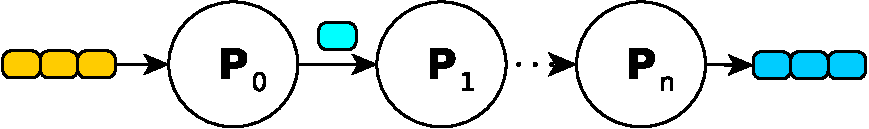
\includegraphics[width=0.40\textwidth]{figures/pipeline.pdf}
    \caption{Patrón Pipeline.}
    \label{fig:chap3:Pipeline}
    \end{figure}
\vspace{0.35cm}
    
    \item \textbf{Farm}: Este patrón computa en paralelo la siguiente función: $f: \alpha \rightarrow \beta$ sobre todos los items que aparecen en la secuencia de entrada. Por lo tanto, para cada elemento $x_i$ en la secuencia de entrada, el patrón Farm entrega el elemento a la secuencia de salida como $f(x_i)$. En este patrón, los cálculos realizados por $f$ para los elementos en el flujo de entrada deben ser completamente independientes entre sí, de lo contrario no pueden procesarse en paralelo. 
    
    \vspace{0.35cm}
    \begin{figure}[htb]
    \centering
    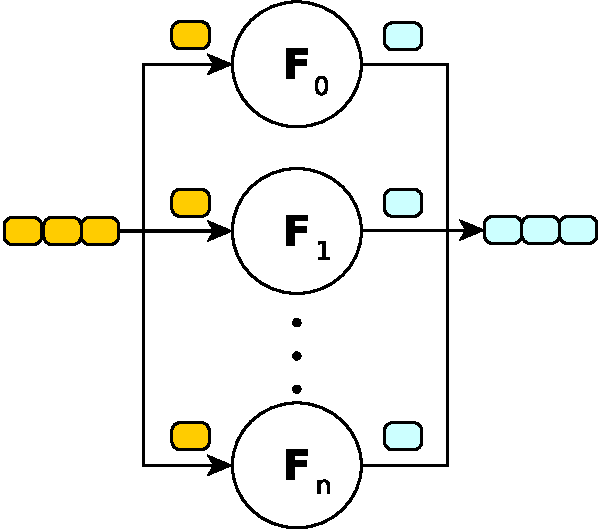
\includegraphics[width=0.30\textwidth]{figures/farm.pdf}
    \caption{Patrón Farm.}
    \label{fig:chap3:Farm}
    \end{figure}
    \vspace{0.35cm}
    
    \item \textbf{Filter}: Este patrón calcula en paralelo un filtro sobre los elementos que aparecen en la secuencia de entrada, pasando solo a la secuencia de salida aquellos elementos que satisfacen la función booleana ``filter'' (o predicado) $\mathcal{P}:\alpha \rightarrow \{true, false\}$. Básicamente, el patrón recibe una secuencia de elementos de entrada $\ldots, x_{i+1}, x_i,$ $x_{i-1}, \ldots$ y produce una secuencia de elementos de salida del mismo tipo pero con diferente cardinalidad. La evaluación de la función de filtrado en un elemento de entrada debe ser independiente de cualquier otra, es decir, el predicado debe ser una función pura. 
    
    \vspace{0.35cm}
    \begin{figure}[htb]
    \centering
    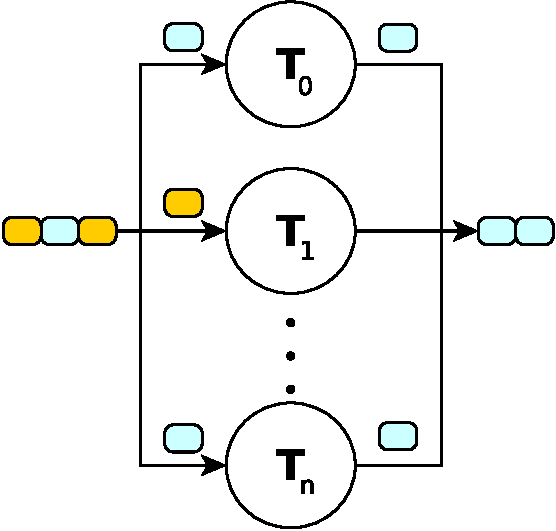
\includegraphics[width=0.30\textwidth]{figures/filter.pdf}
    \caption{Patrón Filter.}
    \label{fig:chap3:filter}
    \end{figure}
    \vspace{0.35cm}
    
    \item \textbf{Accumulator}: Este patrón colapsa los elementos que aparecen en la secuencia de entrada y entrega estos resultados a la secuencia de salida. La función utilizada para contraer los valores de elemento $\oplus$ debe ser una función binaria pura de tipo $\oplus:\alpha \times \alpha \to \alpha$, siendo generalmente asociativa y conmutativa. Básicamente, el patrón calcula la función $\oplus$ sobre una secuencia finita de elementos de entrada $\ldots, x_{i+1}, x_i, x_{i-1}, \ldots$ para producir un elemento contraído en la secuencia de salida . La cantidad de elementos que se acumulará depende del tamaño de ventana configurado como parámetro.
    
    \vspace{0.35cm}
    \begin{figure}[htb]
    \centering
    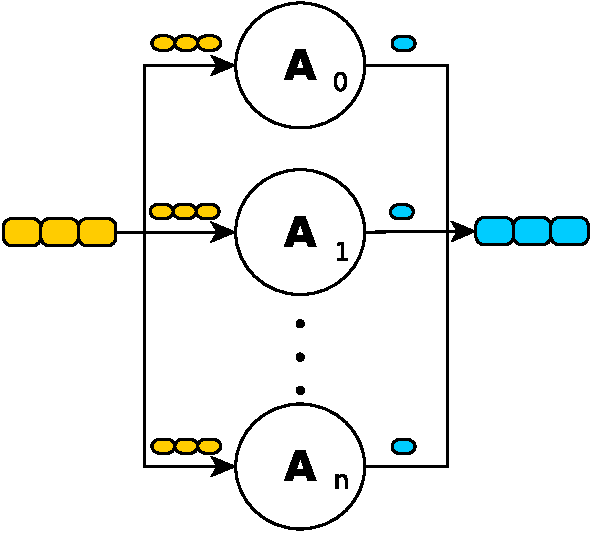
\includegraphics[width=0.30\textwidth]{figures/accumulator.pdf}
    \caption{Patrón Accumulator.}
    \label{fig:chap3:accumulator}
    \end{figure}
    \vspace{0.35cm}
    
\end{itemize}

\subsection{Patrones de datos}

\begin{itemize}
   \item \textbf{Map}: Este patrón paralelo de datos calcula la función $f: \alpha \rightarrow \beta$ sobre los elementos de la colección de datos de entrada, donde los elementos de entrada y salida son de los tipos $\alpha$ y $\beta$ respectivamente. El resultado de salida es la colección de elementos $y_{1}, y_{2}, \ldots, y_{N}$, donde $y_{i} = f(x_{i})$ para cada $i = 1, 2, \ldots, N$ y $x_{i}$ el el elemento $i$-ésimo de la colección de entrada. El único requisito del patrón map es que la función $f$ sea pura. 
   
   \vspace{0.35cm}
   \begin{figure}[htb]
    \centering
    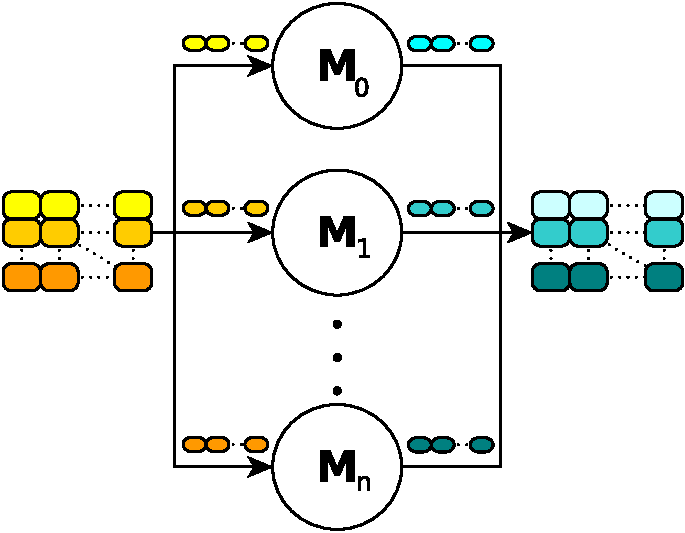
\includegraphics[width=0.35\textwidth]{figures/map.pdf}
    \caption{Patrón Map.}
    \label{fig:chap3:map}
    \end{figure}
    \vspace{0.35cm}
    
    \item \textbf{Reduce}: Este patrón paralelo de datos agrega los elementos de la colección de datos de entrada de tipo $\alpha$ utilizando la función binaria $\oplus: \alpha \times \alpha \to \alpha $, que generalmente es asociativa y conmutativa. Finalmente, el resultado del patrón se resume en un solo elemento $y$ del tipo $\alpha$ que se obtiene al realizar la operación $y = x_{1} \oplus x_{2} \oplus \ldots x_{N}$, donde $x_{i}$ es el elemento $i$-ésimo de la colección de datos de entrada. La principal restricción de este patrón es que la función binaria debe ser pura.
    
    \vspace{0.35cm}
    \begin{figure}[htb]
    \centering
    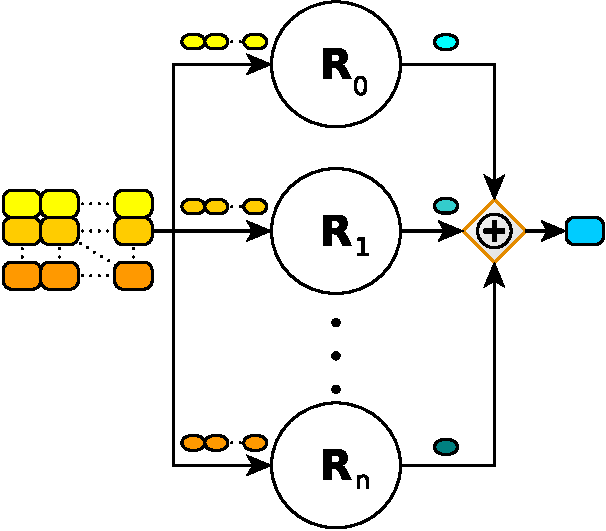
\includegraphics[width=0.3\textwidth]{figures/reduce.pdf}
    \caption{Patrón Reduce.}
    \label{fig:chap3:reduce}
    \end{figure}
    \vspace{0.35cm}

    \item \textbf{Stencil}: Este patrón es una generalización del patrón map en el cual una función elemental puede acceder, no solo a un elemento único en una colección de entrada, sino también a un conjunto de vecinos. La función $f: \alpha* \rightarrow \alpha$ utilizada por el patrón stencil recibe el elemento de entrada y un conjunto de vecinos ($\alpha*$) y produce un elemento de salida del mismo tipo. El principal requisito de este patrón es que la función $f$ debe ser pura. 
    
    \vspace{0.35cm}
    \begin{figure}[htb]
    \centering
    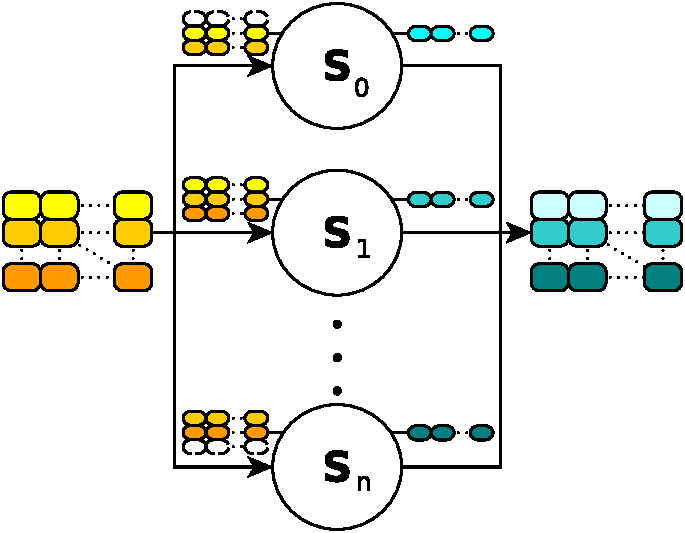
\includegraphics[width=0.35\textwidth]{figures/stencil.pdf}
    \caption{Patrón Stencil.}
    \label{fig:chap3:stencil}
    \end{figure}
    \vspace{0.35cm}
    
    \item \textbf{MapReduce}: Este patrón calcula, en una primera etapa, un patrón tipo map, una función de valor de clave sobre todos los elementos de una colección de entrada, y entrega, en una segunda etapa, un patrón de reducción, un conjunto de pares de valores de clave únicos donde el valor asociado a la clave es la ``suma'' de los valores emitidos para la misma clave. Para hacerlo, el patrón mapreduce calcula en la función map $f : \alpha \rightarrow \{\alpha, Key\}$ los elementos en la colección de entrada; luego usa la función binaria de reducción $\oplus: \beta \times \beta \to \beta$ para resumir los resultados parciales con la misma clave. El resultado de este patrón es una colección de elementos de datos de tipo $\beta$, uno por clave. Los requisitos del patrón mapreduce es que las funciones relacionadas tanto map como reduction deben ser puras.
    
    \vspace{0.35cm}
    \begin{figure}[htb]
    \centering
    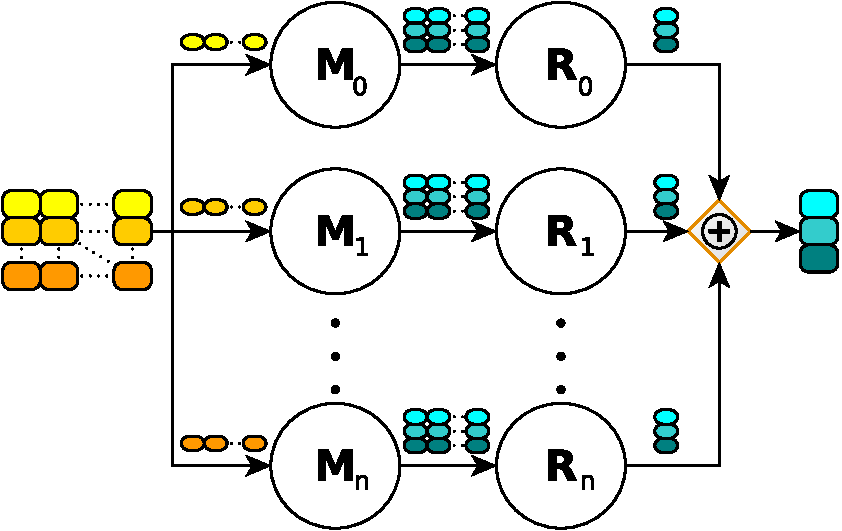
\includegraphics[width=0.40\textwidth]{figures/mapreduce.pdf}
    \caption{Patrón MapReduce.}
    \label{fig:chap3:mapreduce}
    \end{figure}
    \vspace{0.35cm}
    
    \item \textbf{Divide\&Conquer}: Este patrón calcula un problema dividiéndolo en dos o más subproblemas del mismo tipo hasta que se alcanza el caso base y se resuelve directamente. Después, las soluciones de los subproblemas se combinan para proporcionar una solución al problema original. En otras palabras, este patrón aplica la función $f : \alpha * \rightarrow \beta * $ en una colección de elementos de tipo $\alpha$ y produce una colección de elementos de tipo $\beta$. Una función de división $\mathcal{D}$ se usa primero para dividir la colección en distintas particiones hasta el tamaño del problema base, que se puede resolver directamente aplicando $f$. Finalmente, los resultados parciales de los problemas de base se combinan de acuerdo con una función de combinación $\mathcal{M}$ para construir la colección de salida final. Los requisitos del patrón dac es que las funciones $f$, $\mathcal{S}$ y $\mathcal{M}$ deben ser puras. 
    
    \vspace{0.35cm}
    \begin{figure}[htb]
    \centering
    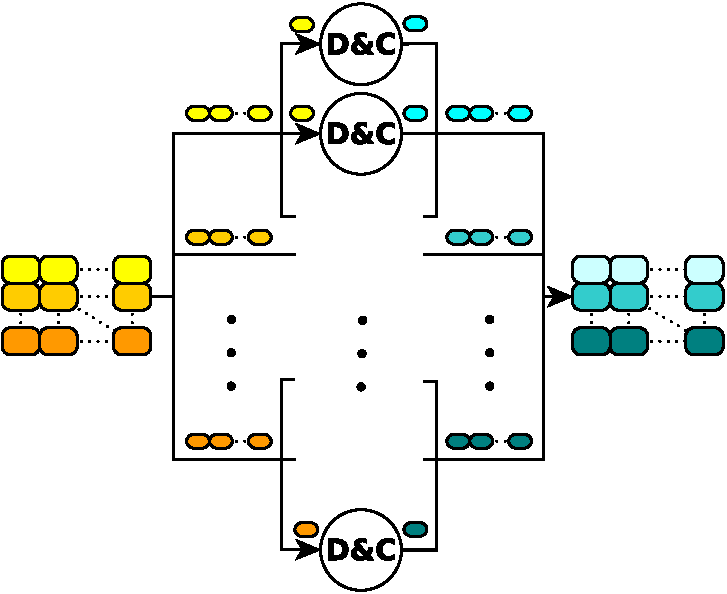
\includegraphics[width=0.40\textwidth]{figures/divideandconquer.pdf}
    \caption{Patrón Divide\&Conquer.}
    \label{fig:chap3:divideandconquer}
    \end{figure}
    \vspace{0.35cm}
    
\end{itemize}

\section{Interfaz de los patrones en \acrshort{grppi}}
\label{sec:interfaz_patrones_grppi}

En esta sección se presenta la interfaz de patrones paralelos genérica y reutilizable (\acrshort{grppi}) para aplicaciones C ++. \acrshort{grppi} aprovecha al máximo las características modernas de C ++, los conceptos de metaprogramación y la programación genérica para actuar como un interruptor entre los modelos de programación paralelos \acrshort{openmp}, hilos C ++, Intel \acrshort{tbb} y \acrshort{cuda} Thrust. Su diseño permite a los usuarios aprovechar los frameworks de ejecución antes mencionados solo en una interfaz única y compacta, ocultando la complejidad detrás del uso de mecanismos de concurrencia. Además, la modularidad de \acrshort{grppi} permite integrar fácilmente nuevos patrones, combinándolos para organizar otros más complejos. Gracias a esta propiedad, \acrshort{grppi} se puede utilizar para implementar una amplia gama de aplicaciones existentes de procesamiento de datos y de flujo de datos con esfuerzos relativamente pequeños, teniendo como resultado códigos portátiles que se pueden ejecutar en múltiples frameworks. La Figura \ref{fig:chap3:grppi} representa la vista general de la biblioteca \acrshort{grppi}.

\vspace{0.35cm}
\begin{figure}[htb]
    \centering
    \includegraphics[width=0.60\textwidth]{figures/grppi.pdf}
    \caption{Arquitectura de \acrshort{grppi}.}
    \label{fig:chap3:grppi}
    \end{figure}
    \vspace{0.35cm}

A continuación, describimos en detalle las interfaces de los patrones paralelos ofrecidos por \acrshort{grppi} y demostrar su capacidad de compilación a través de diferentes ejemplos simples.

\subsection{Descripción de las interfaces}

\acrshort{grppi} ofrece patrones de streaming y patrones de datos con una única interfaz cuidadosamente diseñada para permitir la composición y admitir múltiples back-ends de implementación.

\subsubsection{Patrones de streaming}

Los patrones de streaming incluídos en \acrshort{grppi} son Pipeline, Farm, Filter y Accumulator.

\begin{itemize}
    \item \textbf{Pipeline}: La interfaz \acrshort{grppi} diseñada para el patrón Pipeline recibe el modelo de ejecución y las funciones (\texttt{in} y \texttt{stages}) relacionadas con sus etapas. Como se puede ver en el Listado \ref{code:Pipeline}, su interfaz C ++ usa plantillas, haciéndola más flexible y reutilizable para cualquier tipo de datos. Tenga en cuenta también el uso de plantillas variadicas, lo que permite que una tubería tenga un número arbitrario de etapas al recibir una colección de objetos invocables pasados como argumentos. En \acrshort{grppi}, la implementación paralela de este patrón se lleva a cabo utilizando un conjunto de entidades concurrentes, cada una de las cuales se ocupa de una sola etapa. Esto se controla a través del parámetro del modelo de ejecución, que se puede configurar para operar en secuencia o en paralelo, a través de los diferentes frameworks compatibles; p.ej. para usar \acrshort{openmp}, el parámetro debe establecerse en \texttt{parallel\_execution\_omp}.
    
    \vspace{0.35cm}
    \begin{lstlisting}[frame=single,label={code:Pipeline},caption={Interfaz Pipeline.}]
template <typename ExecMod, typename InFunc, typename ... Arguments>
void Pipeline( ExecMod m, InFunc const &in, Arguments ... stages );
\end{lstlisting}
\vspace{0.35cm}

    \item \textbf{Farm}: De forma similar, la interfaz del patrón Farm, que se muestra en el Listado \ref{code:Farm}, recibe el modelo de ejecución y tres funciones (\texttt{in}, \texttt{Farm} and \texttt{out}) que son a cargo de \emph{i)} consumir los artículos del flujo de entrada, \emph{ii)} procesarlos individualmente, y \emph{iii)} entregar los resultados al flujo de salida. Tenga en cuenta que la función \texttt{Farm} se ejecutará en paralelo por las diferentes entidades concurrentes. En este caso, el modelo de ejecución puede recibir opcionalmente, como argumento, el número de entidades que se utilizarán para la ejecución paralela, por ejemplo, \texttt{parallel\_execution\_omp\{6\}} utiliza 6 hilos de trabajo \acrshort{openmp}. Si no se proporciona este argumento, la interfaz toma por defecto el número de hilos establecidos por la plataforma subyacente.
    
    \vspace{0.35cm}
    \begin{lstlisting}[frame=single,label={code:Farm},caption={Interfaz Farm.}]
template <typename ExecMod, typename InFunc, typename TaskFunc, typename OutFunc>
void Farm( ExecMod m, InFunc const &in, TaskFunc const &Farm, OutFunc const &out );
\end{lstlisting}
\vspace{0.35cm}
    
    \item \textbf{Filter}: La interfaz para el patrón filter, que se describe en el Listado \ref{code:filter}, recibe el argumento del modelo de ejecución, seguido de un consumidor de flujo (\texttt{in}), filtro (\texttt{filter}) y productor (\texttt{out}). Específicamente, la función \texttt{in} lee elementos de la secuencia de entrada y los reenvía a la función \texttt{filter} que es responsable de determinar si un elemento debe ser aceptado o no. Posteriormente, los elementos que satisfacen la rutina de filtrado son recibidos por la función \texttt{out} para entregarlos al flujo de salida. Tenga en cuenta que es obligatorio que la función \texttt{filter} devuelva una expresión booleana. La implementación paralela de este patrón aplica la función de filtro usando un conjunto de entidades concurrentes, que se pueden configurar en el parámetro del modelo de ejecución.
    
    \vspace{0.35cm}
    \begin{lstlisting}[frame=single,label={code:filter},caption={Interfaz Filter.}]
template <typename ExecMod, typename InFunc, typename FilterFunc, typename OutFunc>
void Filter( ExecMod m, InFunc const &in, FilterFunc const &filter, OutFunc const &out );
\end{lstlisting}
\vspace{0.35cm}
    
    \item \textbf{Accumulator}: El patrón accumulator tiene como objetivo reducir, utilizando una función de reducción específica (\texttt{redop}) los elementos que aparecen en el flujo de entrada. De forma similar a las otras interfaces, la interfaz del acumulador, como se muestra en el Listado \ref{code:accum}, recibe el modelo de ejecución; la función de consumidor de flujo (\texttt{in}) el tamaño de la ventana, es decir, el número de elementos que formarán parte de cada operación de reducción; el desplazamiento, que determina el número de elementos superpuestos entre las ventanas; el operador de reducción; y una función de productor (\texttt{out}) responsable de entregar los artículos al flujo de salida. En este caso, las entidades concurrentes en la implementación paralela son responsables de procesar individualmente la acumulación de las ventanas de flujo de entrada.
    
    \vspace{0.35cm}
    \begin{lstlisting}[frame=single,label={code:accum},caption={Interfaz Accumulator.}]
template <typename GenFunc, typename ReduceOperator, typename OutFunc>
void Accumulator( ExecMod m, GenFunc const &in, int windowsize, int offset, ReduceOperator const &redop, OutFunc const &out );
\end{lstlisting}
\vspace{0.35cm}
    
\end{itemize}

\subsubsection{Patrones de datos}

Los patrones de datos incluídos en \acrshort{grppi} son Map, Reduce, Stencil, MapReduce y Divide\&Conquer.

\begin{itemize}
    \item \textbf{Map}: La interfaz \acrshort{grppi} para el patrón map, que se muestra en el Listado~\ref{code:map}, ecibe los siguientes parámetros de entrada: el modelo de ejecución, las referencias al primer y último elemento de las colecciones de datos de entrada y la función kernel (\texttt{map}). Después del cálculo, el resultado del patrón del mapa se deja en la posición correspondiente del conjunto de datos de salida. Dado que cada elemento de la colección de datos de entrada es independiente entre sí, la ejecución paralela del patrón de mapa se puede realizar de la siguiente manera. Primero, la colección de entrada se divide por igual entre las entidades concurrentes disponibles. Posteriormente, estas entidades ejecutan en paralelo la función kernel \texttt{map} y escriben los resultados en los segmentos correspondientes de la recopilación de datos de salida.
    
    \vspace{0.35cm}
    \begin{lstlisting}[frame=single,label={code:map},caption={Interfaz Map.}]
template <typename ExecMod, typename InputIt, typename OutputIt, typename TaskFunc, typename ... MoreIn>
void Map(ExecMod m, InputIt first, InputIt last, OutputIt firstOut, TaskFunc const &map, MoreIn ... inputs );
\end{lstlisting}
\vspace{0.35cm}
    
    \item \textbf{Reduce}: La interfaz para el patrón reduce, como se describe en el Listado~\ref{code:reduce}, toma el modelo de ejecución, una referencia al primer y último elemento de la colección de datos de entrada y al operador de reducción. El resultado de la reducción se escribe en el parámetro de salida pasado por referencia. De acuerdo con las propiedades del operador de reducción, el cálculo de reducción se puede realizar en paralelo. Por lo tanto, la recopilación de datos de entrada se divide en $N$ trozos y se calcula en paralelo mediante $N$ entidades concurrentes diferentes que producen un conjunto de resultados parciales. Finalmente, el resultado del patrón de reducción se calcula en serie por una de estas entidades.
    
    \vspace{0.35cm}
    \begin{lstlisting}[frame=single,label={code:reduce},caption={Interfaz Reduce.}]
template <typename ExecMod, typename InputIt, typename Output, typename ReduceOperator>
void Reduce(ExecMod m, InputIt first, InputIt last, Output &out, ReduceOperator const &redop);
\end{lstlisting}
\vspace{0.35cm}
    
    \item \textbf{Stencil}: La interfaz \acrshort{grppi} para el patrón stencil, presentado en el Listado~\ref{code:stencil}, es bastante similar a la del patrón de mapa, con la excepción de que también recibe la función de vecindad  (\texttt{nh}). Esta función es responsable de acceder a los vecinos en una determinada coordenada del conjunto de datos de entrada. La implementación paralela del patrón de esténcil es análoga a la del patrón de mapa. Sin embargo, el acceso a los vecinos en los límites de un conjunto de datos particionados podría requerir comparaciones adicionales entre las posiciones de los elementos.
    
    \vspace{0.35cm}
    \begin{lstlisting}[frame=single,label={code:stencil},caption={Interfaz Stencil.}]
template <typename ExecMod, typename InputIt, typename OutputIt, typename TaskFunc, typename NFunc, typename ... MoreIn>
void Stencil(ExecMod m, InputIt first, InputIt first, InputIt last, OutputIt firstOut, TaskFunc const &stencil, NFunc const &nh, MoreIn ... inputs);
\end{lstlisting}
\vspace{0.35cm}
    
    \item \textbf{MapReduce}: La interfaz para el patrón mapreduce combina llamadas internas al mapa y reduce las interfaces del patrón \acrshort{grppi}. En cuanto a los parámetros de entrada, recibe el modelo de ejecución, referencias al primer y último elemento de las colecciones de datos de entrada, la función kernel  (\texttt{map}) y el operador de reducción para el patrón reduce. El resultado finalmente se deja en una referencia al primer elemento de la colección de salida. La implementación paralela de este patrón en \acrshort{grppi} explota el paralelismo ofrecido internamente por el mapa y reduce los patrones paralelos. El resultado de la operación del mapa se baraja y se reduce en paralelo, uno para todos los elementos con la misma clave. El resultado global para cada clave finalmente se reduce en serie por una de las entidades concurrentes.
    
    \vspace{0.35cm}
    \begin{lstlisting}[frame=single,label={code:mapreduce},caption={Interfaz MapReduce.}]
template <typename ExecMod, typename InputIt, typename Output, typename MapFunc, typename ReduceOperator, typename ... MoreIn>
void MapReduce(ExecMod m, InputIt first, InputIt last, Output &out, MapFunc const &map, ReduceOperator const &redop, MoreIn ... inputs);
\end{lstlisting}
\vspace{0.35cm}
    
    \item \textbf{Divide\&Conquer}: La interfaz diseñada para el patrón Divide\&Conquer consta de los siguientes elementos: el modelo de ejecución, una referencia de la colección de datos de entrada y las funciones \texttt{divide}, \texttt{base\_case} and \texttt{merge}. El resultado de este patrón se escribe en la recopilación de datos de salida pasada por referencia. La implementación paralela de este patrón en la interfaz \acrshort{grppi} aprovecha primero el núcleo dividido para dividir el problema de manera constante en otros más pequeños. Esta operación es realizada por las entidades concurrentes disponibles hasta que se alcanza la dimensión de problema mínima y donde se aplica el kernel de solución de caso base. Tomando las soluciones parciales generadas, las entidades concurrentes fusionan los resultados en una estructura basada en árbol hasta que se obtiene la solución global. Tenga en cuenta que dado que el ancho del árbol puede crecer por encima del número máximo de entidades concurrentes especificadas, se usa un grupo de tareas para implementar un enfoque de programación dinámica.
    
    \vspace{0.35cm}
    \begin{lstlisting}[frame=single,label={code:dac},caption={Interfaz Divide\&Conquer.}]
template <typename ExecMod, typename Input, typename Output, typename DivFunc, typename TaskFunc, typename MergeFunc>
void DivideAndConquer(ExecMod m, Input &problem, Output &out, DivFunc const &divide, TaskFunc const &base_case, MergeFunc const &merge);
\end{lstlisting}
\vspace{0.35cm}
    
\end{itemize}

\subsection{Composición de patrones}

Como se mencionó previamente, los patrones ofrecidos por \acrshort{grppi} pueden componerse entre ellos para producir estructuras más complejas y para unir construcciones específicas presentes en aplicaciones secuenciales y paralelas de datos. Para demostrar esta característica, describimos tres ejemplos de compibilidad de patrones abordando cada una de las combinaciones factibles de paradigmas computacionales (streaming y datos) soportados por la interfaz \acrshort{grppi}: stream-stream, data-data y composición stream-data.

Para la composición del patrón stream-stream, el código en el Listado\ref{code:stream-stream-comp} implementa un Pipeline en el que la segunda etapa es un patrón Farm. Las etapas del Pipeline, pasadas como funciones lambda, realizan las siguientes tareas: \emph{i)} leer las líneas de un archivo de entrada con valores separados por espacios en blanco y empaquetarlos en una estructura vectorial, \emph{ii)} calcular el valor máximo de vectores entrantes usando el patrón Farm, y \emph{iii)} imprime los valores máximos de los vectores en un flujo de salida. Dado que el Pipeline recibe el modelo de ejecución paralela \acrshort{openmp} (línea 1), las etapas se calculan en paralelo por los 3 hilos de trabajo. De forma similar, el patrón de conjunto anidado se ejecuta mediante 6 hilos \acrshort{openmp}. Tenga en cuenta también que las variables \texttt {std::optional}, de \emph{c++ Library Fundamentals Extensions} (ISO / IEC 19568: 2015), se utilizan para marcar el final de las secuencias con un valor vacío. Denotamos esta composición de Pipeline-Farm \texttt{(\,p\,$|$\,f\,$|$\,p\,)}, siendo \texttt{p} y \texttt{f}, respectivamente, etapas secuenciales y basadas en Farm. Como se puede ver, gracias al uso de técnicas de metaprogramación, plantillas y expresiones lambda, es posible componer fácilmente patrones paralelos \acrshort{grppi} para construir otros más complejos.

\vspace{0.35cm}
\begin{lstlisting}[frame=single,label={code:stream-stream-comp},caption={Ejemplo de composición Pipeline-Farm.}]
Pipeline( parallel_execution_omp,
    // Stage 0: read values from a file
    [&]() -> optional<vector<int>> {
        auto r = read_list(is);
        return ( r.size() == 0 ) ? {} : r; 
    },
    // Stage 1: takes the maximum value of the vector
    Farm(parallel_execution_omp{6}, 
        []( vector<int> v ) {
            return ( v.size() > 0 ) ? 
                max_element(v.begin(), v.end()) : 
                numeric_limits<int>::min();
    }),
    //Stage 2: prints out the result
    [&os]( int x ) {
        os << x << endl;
    }
);
\end{lstlisting}
\vspace{0.35cm}

Con respecto a la composición del patrón de datos de datos, el Listado~\ref{code:data-data-comp} muestra una construcción donde se compone un patrón map con una operación reduce. En este caso, la matriz de entrada en el patrón map se divide en particiones iguales entre los hilos del trabajador. A continuación, para cada fila en una partición, el patrón reduce anidado resume sus valores y almacena el resultado en la posición correspondiente del vector de salida, pasado como un argumento en la llamada a la función del map. Tenga en cuenta que el modelo de ejecución en paralelo para el patrón map es \acrshort{openmp}, mientras que el patrón reduce anidado utiliza subprocesos de C ++, cada uno de ellos utilizando 6 subprocesos de trabajo. Denotamos esta composición como \texttt{m(r)}, siendo \texttt{m} y \texttt{r} los patrones map y reduce, respectivamente.

\vspace{0.35cm}
\begin{lstlisting}[frame=single,label={code:data-data-comp},caption={Ejemplo de composición Map-Reduce.}]
Map( parallel_execution_omp{6},
    // Input matrix
    mat_in.begin(), mat_in.end(),
    // Vector of accumulated values from matrix rows
    vec_out.begin(),
    // Map kernel: divide matrix into rows
    [&]( auto row_in, auto sum ) {
        // Reduce kernel: Sum up the values in a matrix row
        Reduce( parallel_execution_thr{6},
            row_in.begin(), row_in.end(), 
            &sum, 
            std::plus<double> );
        );
    }
);
\end{lstlisting}
\vspace{0.35cm}

Como se mencionó, también podemos componer stream con patrones de datos. Esta es una composición factible, dado que los elementos provenientes de un flujo se pueden procesar utilizando un patrón paralelo de datos. Sin embargo, lo contrario no es factible ya que los resultados generados en un patrón de datos no pueden transformarse en flujo y, por lo tanto, procesarse utilizando un enfoque de procesamiento de streaming. Para ilustrar una composición de patrón de datos de flujo, el Listado~\ref{code:stream-data-comp} muestra un ejemplo donde un patrón paralelo de flujo de granja se compone con un dato de Divide\&Conquer. En este caso particular, el patrón de Farm lee constantemente los valores almacenados en un archivo y calcula, para cada uno de ellos, su correspondiente \emph{i}-ésimo número de Fibonacci utilizando el patrón Divide\&Conquer. Finalmente, los números de Fibonacci se imprimen para el usuario final. Como se muestra, la paralelización de la granja se realiza utilizando 6 hilos \acrshort{openmp}, mientras que el patrón Divide\&Conquer anidado usa 6 hilos C ++. Dado que cada uno de los subprocesos relacionados con la granja crean 6 anidados en C ++, el número total de subprocesos que computan esta composición es 36. Esta composición se denota como \texttt{f(d)}, siendo \texttt{f} y \texttt{d}, los patrones Farm y Divide\&Conquer, respectivamente.

\vspace{0.35cm}
\begin{lstlisting}[frame=single,label={code:stream-data-comp},caption={Ejemplo de composición Farm-Divide\&Conquer.}]
Farm(parallel_execution_omp(6),
    [&]() -> optional<int> {  // Read values from an input file
        auto value = read_value(is);
        return ( value > 0 ) ? value : {};
    },
    [&]( int value ) { // Compute the fibonacci number using a D&C pattern    
        int fibonacci = 0;
        DivideAndConquer(parallel_execution_thr(6), value, &fibonacci,
            [&](auto &value){
                std::vector< int > subproblem;
                if( v < 2 ) subproblem.push_back(value);
                else        subproblem.insert(subproblem.end(), { value-1, value-2 });
                return subproblem;
            },
            [&](auto &problem, auto &partial){
                partial = ( problem == 0 ) ? 0 : 1;
            },
            [&](auto & partial, auto & out){
                out += partial;
            }
        );
        return fibonacci;
    },
    [&]( int fibonacci ) {  // Print the fibonacci values 
        cout << fibonacci << endl;
    }
);
\end{lstlisting}
\vspace{0.35cm}

En general, las Tablas ~\ref{tab:stream-stream-comp}, ~\ref{tab:data-data-comp} y ~\ref{tab:stream-data-comp} resumen las composiciones de patrones agrupadas por las tres posibles combinaciones de paradigmas computacionales compatibles con la interfaz \acrshort{grppi}: stream-stream, data-data y stream-data. Tenga en cuenta que las filas y columnas en las tablas representan los patrones externos e internos involucrados en una composición determinada, respectivamente. Clasificamos cada composición de patrón específico con una de las siguientes cuatro categorías, desde menos hasta más restrictivas:

\begin{itemize}
    \item \textbf{No-Factible}: Esta categoría representa una composición que no es compatible con \acrshort{grppi}.
    \item \textbf{Factible}: Esta categoría denota una composición que se puede implementar en \acrshort{grppi}.
    \item \textbf{Irreducible}: esta categoría es una composición factible que proporciona un patrón paralelo útil que no puede simplificarse más. Tenga en cuenta que las composiciones de patrones que se incluyen en esta categoría son compatibles de forma nativa con \acrshort{grppi}.
    \item \textbf{Usable-Reducible}: Esta categoría es una composición factible que implementa una composición de patrones que puede simplificarse aún más, pero que, en algunos casos, proporciona un código más claro y más legible que su equivalente más simple.
\end{itemize}

Como se muestra en la Tabla~\ref{tab:stream-stream-comp}, las composiciones de patrones stream-stream que involucran un Pipeline y otro patrón se clasifican como Irreducible (excepto aquellos con un patrón de accumulator externo), dado que no es posible obtener la misma construcción paralela usando un patrón más simple. Este tipo de composiciones son compatibles nativamente en \acrshort{grppi}, como se muestra en el Listado~\ref{code:stream-stream-comp}. Cualquier otra composición se considera Factible ya que pueden simplificarse usando el patrón externo o interno con un mayor grado de paralelismo. Sin embargo, estas construcciones no proporcionan ninguna ventaja importante en comparación con la construcción más simple. Por otro lado, las composiciones que contienen un patrón de acumulador externo son No-Factible, ya que este patrón no recibe ninguna función de usuario para ejecutarse en paralelo.

\vspace{0.35cm}
\begin{table}[htbp]
\centering
%\resizebox{\textwidth}{%
\caption{Composiciones stream-stream.}
\begin{adjustbox}{max width=\textwidth}
\begin{tabular}{@{}ccccc@{}}
\toprule
 & Pipeline & Farm & Filter & Accumulator \\ 
\midrule
Pipeline  & \feasim     & \irredm     & \irredm     & \irredm     \\
\midrule
Farm      & \irredm     & \feasim     & \feasim     & \feasim     \\
\midrule
Filter    & \irredm     & \feasim     & \feasim     & \feasim     \\
\midrule
Accumulator     & \nfeasm     & \nfeasm     & \nfeasm     & \nfeasm     \\
\bottomrule
\end{tabular}
\end{adjustbox}
\label{tab:stream-stream-comp}
\end{table}
\vspace{0.35cm}


Centrándose en las composiciones de datos de datos, como se muestra en la Tabla~\ref{tab:data-data-comp}, las construcciones cuyo patrón exterior es similar a un map (map and stencil) se categorizan como Usable-Reducible. Esto se debe a que existe un equivalente más simple que usa solo el patrón externo tipo mapa. En cuanto al patrón de reducción, no se puede combinar con ningún otro interno. Las razones son las mismas que para el patrón del acumulador en las composiciones de flujo continuo. Otras composiciones cuyo patrón exterior es mapreduce o Divide\&Conquer se clasifican como Factible, ya que pueden implementarse en \acrshort{grppi} aunque no aportan ninguna ventaja importante.

\vspace{0.35cm}
\begin{table}[htbp]
\centering
%\resizebox{\textwidth}{%
\caption{Composiciones data-data.}
\begin{adjustbox}{max width=\textwidth}
\begin{tabular}{@{}cccccc@{}}
\toprule
 & Map       & Reduce    & Stencil   & MapReduce & Divide\&Conquer      \\
\midrule
Map       & \usablm     & \usablm     & \usablm     & \usablm     & \usablm     \\
\midrule
Reduce    & \nfeasm     & \nfeasm     & \nfeasm     & \nfeasm     & \nfeasm     \\
\midrule
Stencil   & \usablm     & \usablm     & \usablm     & \usablm     & \usablm     \\
\midrule
MapReduce & \feasim     & \feasim     & \feasim     & \feasim     & \feasim     \\
\midrule
Divide\&Conquer & \feasim     & \feasim     & \feasim     & \feasim     & \feasim     \\
\bottomrule
\end{tabular}
\end{adjustbox}
\label{tab:data-data-comp}
\end{table}
\vspace{0.35cm}

Finalmente, las composiciones de stream-data se resumen en la Tabla~\ref{tab:stream-data-comp}. Las composiciones cuyo patrón exterior es Pipeline o Farm se denotan como Irreducible. La combinación de dos paradigmas paralelos distintos (stream-data) hace que estas composiciones sean únicas e impide que se simplifiquen más. En cuanto a las composiciones con un patrón de filtro externo, la cardinalidad de salida de su patrón interno determina si la composición es Factible or Usable-Reducible. Esto se debe a que la salida de la función de filtro es booleana. 

\vspace{0.35cm}
\begin{table}[htbp]
\centering
%\resizebox{\textwidth}{%
\caption{Composiciones stream-data.}
%\resizebox{\textwidth}{!}{
\begin{adjustbox}{max width=\textwidth}
\begin{tabular}{@{}cccccc@{}}
\toprule
 & Map       & Reduce    & Stencil   & MapReduce & Divide\&Conquer      \\
\midrule
Pipeline  & \irredm     & \irredm     & \irredm     & \irredm     & \irredm     \\
\midrule
Farm      & \irredm     & \irredm     & \irredm     & \irredm     & \irredm     \\
\midrule
Filter    & \feasim     & \feasim*    & \feasim     & \feasim     & \feasim*    \\
\midrule
Accumulator & \nfeasm     & \nfeasm     & \nfeasm     & \nfeasm     & \nfeasm     \\
\bottomrule
\end{tabular}
\end{adjustbox}
%}
\label{tab:stream-data-comp}
\end{table}
\vspace{0.35cm}

Por ejemplo, en una composición map-filter, la cardinalidad de salida del patrón map es igual a la cardinalidad de entrada. De modo que, aunque el predicado del patrón filter se puede implementar transformando el conjunto de datos de salida en un booleano, este caso no refleja una práctica común. Por lo tanto, clasificamos estas composiciones solo como Factible. Por otro lado, la cardinalidad de salida del patrón reduce en una composición filter-reduce es un elemento único. Por lo tanto, el predicado de filtro se puede implementar fácilmente transformando dicho elemento en un booleano. Por esta razón, categorizamos esta construcción como un caso especial de composición Factible. La combinación filter-Divide\&Conquer también es un caso especial de composición Factible porque la cardinalidad de salida del patrón Divide\&Conquer depende del algoritmo. Finalmente, el patrón accumulator no se puede componer y, por lo tanto, es clasificado como No-Factible.





%\afterpage{\blankpage} % blank page

\lhead[\thepage]{CAPÍTULO \thechapter. INTERFAZ DE PATRONES DE PROG\acrshort{ram}ACIÓN PARALELA PARA MEMORIA DISTRIBUIDA}
\chead[]{}
\rhead[Patrones de programación paralelos de alto nivel en arquitecturas de memoria distribuida\leftmark]{\thepage}
\renewcommand{\headrulewidth}{0.5pt}

\lfoot[]{}
\cfoot[]{}
\rfoot[]{}
\renewcommand{\footrulewidth}{0pt}

%% This is an example first chapter.  You should put chapter/appendix that you
%% write into a separate file, and add a line \include{yourfilename} to
%% main.tex, where `yourfilename.tex' is the name of the chapter/appendix file.
%% You can process specific files by typing their names in at the 
%% \files=
%% prompt when you run the file main.tex through LaTeX.
\chapter{Interfaz de patrones de programación paralela para memoria distribuida}
\label{ch:interfaz_patrones_memoria_distribuida}
\markboth{}{INTERFAZ DE PATRONES DE PROG\acrshort{ram}ACIÓN PARALELA PARA MEMORIA DISTRIBUIDA}

Este capítulo presenta la implementación realizada de \acrshort{grppi} para plataformas de memoria distribuida. En primer lugar se describe el problema (Sección \ref{sec:descripcion_problema}) por el cual se decide realizar esta implementación. Posteriormente, se describe la política de ejecución \acrshort{mpi} para \acrshort{grppi} (Sección \ref{sec:politica_ejecucion_mpi}), describiendo la interfaz de usuario resultante (Sección \ref{sec:interfaz_usuario}), la implementación de las colas de comunicación entre procesos (Sección \ref{sec:colas_comunicacion}) y el algoritmo de distribución de operadores en procesos \acrshort{mpi} (Sección \ref{sec:algoritmo_distribucion_mpi}).

\section{Descripción del problema}
\label{sec:descripcion_problema}

En general, la implementación de un back-end distribuido mediante \acrshort{mpi} se ha motivado principalmente por las necesidades de escalamiento y el desarrollo de nuevos modelos de programación para aplicaciones científicas \acrshort{dasp}. El interés de implementar este back-end proviene de la amplia adopción de \acrshort{mpi} en las supercomputadoras de hoy, que actualmente no tiene soporte estándar para el procesamiento de streaming~\cite{peng2017}. Debido a este motivo al crecimiento en los últimos años del paradigma del \emph{Big Data}, creemos necesario presentar un back-end que pueda ser de ayuda en el desarrollo de aplicaciones de streaming en C ++.

Por otro lado, una vez analizado el estado de la cuestión y las herramientas y frameworks actualmente disponibles para este área, identificamos una brecha importante entre la comunidad de \acrshort{mpi} y las necesidades de procesamiento de flujo de las aplicaciones científicas actuales ~\cite{stream2016}. En este sentido, el objetivo del nuevo back-end de \acrshort{grppi} \acrshort{mpi} es doble. Por un lado, \acrshort{grppi} ofrece una interfaz C ++ de alto nivel de patrones paralelos que mejora tanto la flexibilidad de la aplicación como la legibilidad del código fuente. Por otro lado, el uso de \acrshort{grppi} \acrshort{mpi} permite de forma transparente la ejecución de la aplicación de C ++ en tiempo real en plataformas \acrshort{hpc} distribuidas, ya que \acrshort{grppi} oculta la complejidad relacionada con la comunicación y la sincronización de procesos.

\section{Política de ejecución \acrshort{mpi} para \acrshort{grppi}}
\label{sec:politica_ejecucion_mpi}

Con respecto a la interfaz de patrones paralelos, hemos aprovechado \acrshort{grppi}, una interfaz de patrones paralelos genérica y reutilizable para aplicaciones C ++. Esta interfaz aprovecha al máximo las características modernas de C ++, los conceptos de metaprogramación y la programación genérica para actuar como un interruptor entre , hilos de C ++ y los modelos de programación paralela de Intel \acrshort{tbb}.  Su diseño permite a los usuarios aprovechar los marcos de ejecución antes mencionados en una interfaz única y compacta, ocultando la complejidad detrás del uso de mecanismos de concurrencia. Además, la modularidad de \acrshort{grppi} permite integrar fácilmente nuevos patrones, combinándolos para organizar construcciones más complejas. Además, permite la integración de nuevas políticas de ejecución basadas en modelos de programación distribuidos y de memoria compartida. Gracias a estas propiedades, \acrshort{grppi} se puede utilizar para implementar una amplia gama de aplicaciones existentes de procesamiento de datos y de streaming con esfuerzos relativamente pequeños, teniendo como resultado códigos portátiles que se pueden ejecutar en múltiples plataformas.

Como se indicó anteriormente, el objetivo de \acrshort{grppi} es acomodar una capa de patrones paralelos entre desarrolladores y marcos de programación paralelos existentes. Hasta ahora, \acrshort{grppi} solo admite políticas de ejecución de memoria compartida, como C + + Threads, e Intel \acrshort{tbb}. Para extender \acrshort{grppi} a fin de admitir plataformas distribuidas, hemos incorporado la política de ejecución de \acrshort{mpi} que, en este momento, permite a los usuarios ejecutar los patrones de oleoductos y flujos de granja en clusters de múltiples núcleos. En esta sección, describimos en detalle los elementos básicos de la política de ejecución de \acrshort{mpi}: \emph{i)} interfaz de usuario; \emph{ii)} canales de comunicación interna; y \emph{iii)} algoritmo de distribución de operadores.

\subsection{Interfaz de usuario}
\label{sec:interfaz_usuario}

Dado el diseño \acrshort{grppi}, donde cada política de ejecución se implementa utilizando una clase C ++, para la nueva política \acrshort{mpi} también diseñamos su clase. Esto se debe a que cada una de estas clases contiene las implementaciones de patrones específicos del marco junto con los parámetros de configuración para esa política. Básicamente, las interfaces de patrones \acrshort{grppi} están sobrecargadas con una implementación diferente para cada una de las políticas de ejecución disponibles. Con él, cuando se compila el código de usuario, la implementación del patrón específico se selecciona dependiendo de la política de ejecución pasada como argumento (ver parámetro \texttt{execution\_policy} en la interfaz del patrón Pipeline en la Figura \ref{fig:grppi-Pipeline-pattern}). El Listado~\ref{lst:parallel-exec-mpi} muestra un extracto de la clase de política de ejecución de \acrshort{mpi}. Tenga en cuenta que hemos utilizado la biblioteca Boost \acrshort{mpi} \cite{boost-mpi} como interfaz de C ++ \acrshort{mpi}. 

Como se observa, los constructores de políticas de ejecución reciben los argumentos del programa o el comunicador \acrshort{mpi} directamente. Para admitir escenarios híbridos, ambos constructores pueden recibir una política de ejecución de memoria compartida local. Esta política local se usará para ejecutar múltiples etapas de Pipeline o réplicas de Farm (también denominadas operadores de flujo) dentro del mismo proceso. Por lo tanto, los operadores asignados al mismo proceso se ejecutarán en forma secuencial o en paralelo según la política de ejecución de la memoria compartida seleccionada. 

\vspace{0.35cm}
%\vspace{-0.2cm}
\begin{lstlisting}[linewidth=1\columnwidth,caption={Clase de política de ejecución \acrshort{mpi} en \acrshort{grppi}.},label=lst:parallel-exec-mpi,frame=single]
template<typename LocalPolicy = parallel_execution_native>
class parallel_execution_mpi {
 namespace mpi = boost::mpi;
 ...
 public:
  parallel_execution_mpi(int argc, char** argv, 
          LocalPolicy local_exec_policy = parallel_execution_native{});
  parallel_execution_mpi(mpi::communicator mpi_comm = mpi::communicator{}, LocalPolicy local_exec_policy = parallel_execution_native{});
  ...                           
};
\end{lstlisting}
\vspace{0.35cm}

Como se muestra en el Listado~\ref{lst:Pipeline-example}, el patrón de Pipeline \acrshort{grppi} aprovecha la nueva clase de política de ejecución \acrshort{mpi} para su ejecución. Tenga en cuenta que la política se construye en la declaración utilizando los argumentos \texttt{argc} y \texttt{argv}. Esta canalización consta de tres etapas en la forma \texttt{(p|f|p)}, donde la primera y la tercera etapa se ejecutan en serie, mientras que la segunda ejecuta dos réplicas del mismo operador utilizando el patrón de la granja. Suponiendo que el programa se ejecute mediante 4 procesos de \acrshort{mpi}, el primero y el último respectivamente ejecutan las etapas de generador y consumidor, mientras que el segundo y el tercero calcularán cada una de las réplicas de conjunto. Es importante destacar que los artículos que transitan de una etapa a otra se envían y reciben a través de las colas de comunicación \acrshort{mpi} implementadas dentro de la política de respaldo.

\vspace{0.35cm}
\begin{lstlisting}[linewidth=1\columnwidth,caption={Ejemplo de Pipeline \acrshort{grppi} distribuido.},label={lst:Pipeline-example},frame=single]
grppi::parallel_execution_mpi ex{argc, argv};
grppi::Pipeline(ex, 
  [x=1,n]() mutable -> optional<double> { 
    if (x<=n) return x++;
    else return {}; 
  },
  grppi::Farm(2,[](double x) {
    return x*x;
  }),
  [](double x) { cout << x << endl; }
);
\end{lstlisting}
\vspace{0.35cm}

Los Listados~\ref{fig:grppi-Pipeline-pattern}, ~\ref{fig:grppi-Farm-pattern} muestra los prototipos C ++ \acrshort{grppi} \acrshort{mpi} de los patrones Pipeline y Farm. Tenga en cuenta el uso de \texttt{templates} con parámetros únicos y múltiples (pack) como referencias universales, lo que permite pasar múltiples objetos invocables (por ejemplo, un functor o expresión lambda) como para los operadores de patrones. Tenga en cuenta también que el primer parámetro indica la política de ejecución que se utilizará para ejecutar los operadores.

\vspace{0.35cm}
\begin{lstlisting}[linewidth=1\columnwidth,caption={Interfaz patrón Pipeline en \acrshort{grppi} \acrshort{mpi}.},label={fig:grppi-Pipeline-pattern},frame=single]
template <typename E, typename G, typename ... O>
void Pipeline(E execution_policy, G && generator, O && ... operators);
\end{lstlisting}
\vspace{0.35cm}

\begin{lstlisting}[linewidth=1\columnwidth,caption={Interfaz patrón Farm en \acrshort{grppi} \acrshort{mpi}.},label={fig:grppi-Farm-pattern},frame=single]
template <typename O>
void Farm(int replicas_replicas, O && operators);  
\end{lstlisting}
\vspace{0.35cm}

\subsection{Colas de comunicación}
\label{sec:colas_comunicacion}

Los canales de comunicación son fundamentales en las aplicaciones de \acrshort{dasp} distribuidas. Por ejemplo, el operador de flujo que se ejecuta en un nodo necesita recibir elementos del operador anterior mapeado en otro nodo, realizar algunos cálculos sobre ellos y enviarlos al próximo operador. Por lo tanto, para habilitar el paralelismo de flujo entre nodos en la política de ejecución \acrshort{mpi}, determinamos la necesidad de canales de comunicación en forma de colas Primero en entrar, primero en salir (FIFO). Para eso, dado que \acrshort{mpi} no admite de forma nativa las colas distribuidas, hemos proporcionado una cola de comunicación unidireccional sobre las primitivas \acrshort{mpi} \texttt{send} y \texttt{receive}, es decir, las comunicaciones a dos caras. Básicamente, estas colas encapsulan las comunicaciones entre procesos \acrshort{mpi} que ejecutan operadores de flujo. De esta forma, las implementaciones de patrones solo hacen uso de las funciones públicas de cola, por ejemplo, el lado del productor de cola \acrshort{mpi} llama \texttt{push} para poner en la cola un elemento que debe enviarse al siguiente operador; mientras que el lado del consumidor llama a \texttt{pop} para desencolar un elemento al recibirlo del operador anterior.

Teniendo en cuenta las posibles disposiciones entre patrones \acrshort{grppi} Pipeline y Farm, identificamos cuatro escenarios de comunicación diferentes:
\begin{itemize}
\item \emph{Single-Producer, Single-Consumer} (SPSC): dos etapas Pipeline consecutivas \texttt{(p|p)}.
\item \emph{Single-Producer, Multiple-Consumer} (SPMC): una etapa de Pipeline a un conjunto de réplicas de Farm \texttt{(p|f)}.
\item \emph{Multiple-Producer, Single-Consumer} (MPSC): un conjunto de réplicas de Farm a una etapa de Pipeline \texttt{(f|p)}.
\item \emph{Multiple-Producer, Multiple-Consumer} (MPMC): un conjunto de réplicas de Farm a otro conjunto de réplicas de Farm \texttt{(f|f)}. 
\end{itemize}

\vspace{0.35cm}
\begin{figure}[!tbp]
\centering
\begin{subfigure}[b]{.5\textwidth}
  \centering
  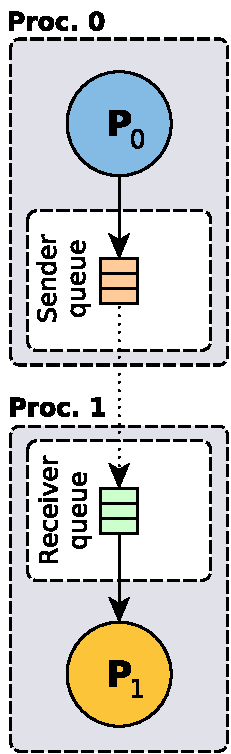
\includegraphics[width=0.3\linewidth]{figures/mpi-spsc-queue.pdf}
  \caption{Diagrama de colas SPSC.}
  %\label{fig:sub1}
\end{subfigure}%
\hfill
\begin{subfigure}[b]{.5\textwidth}
  \centering
  \includegraphics[width=0.5\linewidth]{figures/mpi-spsc-communication.pdf}
  \caption{Protocolo de comunicación de colas SPSC.}
  %\label{fig:sub2}
\end{subfigure}
\caption{Diagrama y protocolo de comunicación de colas SPSC.}
\label{fig:spsc-queue}
\end{figure}
\vspace{0.35cm}

El lado izquierdo de las Figuras ~\ref{fig:spsc-queue} y~\ref{fig:mpmc-queue} muestran, respectivamente, los diagramas de cola en los escenarios de SPSC y MPMC.\footnote{Consideramos el SPMC y MPSC los escenarios se implementan utilizando el modo de cola MPMC, ya que estos casos se pueden ver como especializaciones de MPMC.} Como se muestra en el lado del productor de colas MPMC, la cola crea un subproceso de controlador por proceso de productor ($T$) para solapar las comunicaciones con los cálculos del operador. La cola también selecciona un hilo del controlador que actúa como el orquestador, que es responsable de gestionar la cola haciendo un seguimiento de los artículos disponibles en cada productor y reenviando las solicitudes de artículos de consumo a un productor determinado. Sin embargo, para la cola de SPSC, dado que los procesos de productor y consumidor son conocidos de antemano, las comunicaciones pueden superponerse con cálculos utilizando directamente primitivas de envío/recepción asíncronas de \acrshort{mpi}. Por lo tanto, no se necesitan subprocesos de controlador en el lado del productor para administrar la cola cuando se trata de escenarios de SPSC.

Para implementar el comportamiento mencionado anteriormente, los lados de cola de \acrshort{mpi} del productor y del consumidor se comunican siguiendo un protocolo específico dependiendo del modo de cola ((ver lado derecho de las Figuras~\ref{fig:spsc-queue} y~\ref{fig:mpmc-queue} para SPSC y MPMC, respectivamente). Este protocolo de comunicación se compone de las tres fases siguientes:

\begin{itemize}
\item \textbf{Fase de configuración}: el objetivo de esta fase es determinar si la cola debe ejecutarse en modo SPSC o MPMC. Si solo hay un productor y un consumidor, entonces la cola se configura como SPSC; de lo contrario, se establece como MPMC. Al comienzo de esta fase, tanto productores como consumidores inicializan sus lados de cola de acuerdo con el tipo de operador (etapa de Pipeline o réplica de Farm). A partir de este momento, todos los procesos intercambian diferentes mensajes de configuración con el proceso del orquestador para seleccionar el modo de cola. Primero, los consumidores y productores respectivamente envían los mensajes \texttt{reg\_recv<id, type>} y \texttt{reg\_send<id>} para registrarse en el orquestador. Además, los consumidores indican el orquestador su \texttt{type}, es decir, la etapa de Pipeline o la réplica de Farm. A continuación, el orquestador configura la cola como SPSC o MPMC según la cantidad de consumidores y productores registrados, y les comunica el modo de cola final (\texttt{ack<mode>}). Finalmente, los procesos de los productores inician los hilos de controlador correspondientes si la cola está configurada como MPMC.

\item \textbf{Fase de comunicación}: se usa un protocolo de comunicación diferente dependiendo del modo de cola. Si la cola está configurada como SPSC, el proceso del productor envía los artículos de manera asíncrona al consumidor. De lo contrario, si la cola está configurada en modo MPMC, el hilo del orquestador espera mensajes provenientes de productores y consumidores. Los productores envían mensajes \texttt{notify\_item<id>} para informar sobre un nuevo artículo disponible, mientras que los consumidores envían \texttt{item\_req<id>} para pedirle al orquestador un artículo. Cuando el orquestador recibe una nueva solicitud, sirve el artículo directamente o reenvía la solicitud a otro productor, siguiendo el mismo orden en el que llegaron las notificaciones del productor.

\vspace{0.35cm}
\begin{figure}[!tbp]
\centering
\begin{subfigure}[b]{0.5\textwidth}
  \centering
  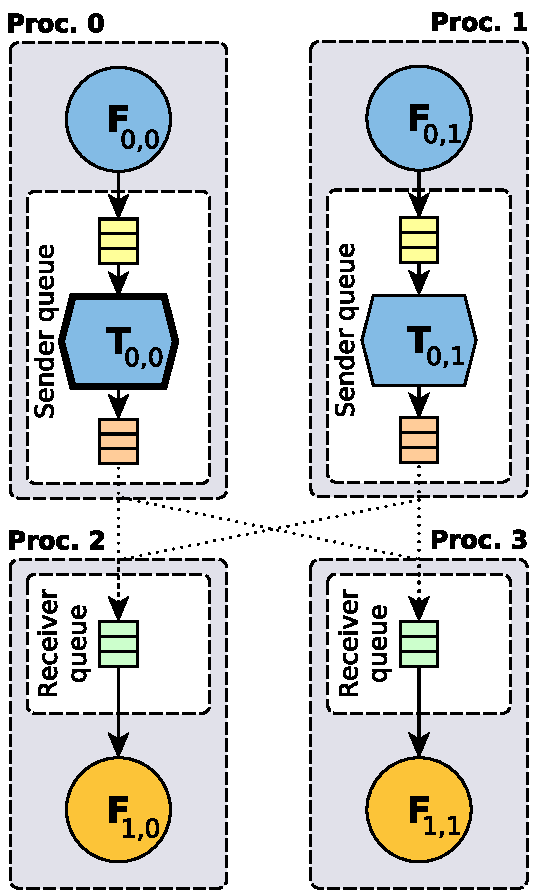
\includegraphics[width=0.55\linewidth]{figures/mpi-mpmc-queue.pdf}
  \caption{Diagrama de colas MPMC.}
  \label{fig:sub1}
\end{subfigure}%
\hfill
\begin{subfigure}[b]{0.5\textwidth}
  \centering
  \includegraphics[width=0.95\linewidth]{figures/mpi-mpmc-communication.pdf}
  \caption{Protocolo de comunicación de colas MPMC.}
  \label{fig:sub2}
\end{subfigure}
\caption{Diagrama y protocolo de comunicación de colas MPMC.}
\label{fig:mpmc-queue}
\end{figure}
\vspace{0.35cm}

\item \textbf{Fase de finalización}: Similar a la fase anterior, se usa un protocolo de terminal diferente dependiendo del modo de cola. Para el modo SPSC, tan pronto como el productor finaliza su operación, envía el mensaje \emph{end-of-stream} (\texttt{EOS}) al consumidor. Por el contrario, para el modo MPMC, el orquestador espera mensajes de \texttt{EOS} de todos los productores, incluido su propio elemento de terminación. Cuando esto sucede, el orquestador envía a cada uno de los consumidores el mensaje \texttt{EOS} para finalizar la comunicación.
\end{itemize}

Gracias a estas colas, los operadores de stream ejecutados por procesos \acrshort{mpi} pueden transmitir elementos de acuerdo con el flujo de stream dictado por una construcción de Pipeline concreta, que puede estar compuesta por diferentes patrones de Farm. Tenga en cuenta que si un proceso utiliza varias instancias de cola simultáneamente, las etiquetas \acrshort{mpi}, en lugar de múltiples comunicadores, se utilizan para hacer referencia a cada una de ellas.

\subsection{Algoritmo de distribución de operadores en procesos \acrshort{mpi}}
\label{sec:algoritmo_distribucion_mpi}

La política de ejecución de \acrshort{mpi} también incorpora un algoritmo de asignación para asignar operadores de flujo en procesos \acrshort{mpi}. Básicamente, este algoritmo calcula al comienzo de la ejecución de la tubería la cantidad total de operadores involucrados en ella, considerando tanto el número de etapas como las réplicas de la granja. Luego, calcula la cantidad de operadores que se deben ejecutar por proceso de \acrshort{mpi} ($opp$). Por defecto, los operadores se distribuyen homogéneamente usando la fórmula:

\vspace{0.35cm}
\begin{equation}\label{eq:opp}
opp= \frac{num\_ops}{num\_procs}
\end{equation}
\vspace{0.35cm}

Sin embargo, el usuario puede anular este valor llamando a la función \texttt{set\_grouping\_granularity(int ops\_per\_proc)}, parte de la clase de política de ejecución de \acrshort{mpi}. A continuación, cada uno de los procesos de \acrshort{mpi} calcula, utilizando su rango, el rango de operadores que deberían ejecutarse con la siguiente fórmula:

\vspace{0.35cm}
\begin{gather}\label{eq:range}
  Range(rank) =
  \begin{cases}
  \{rank * opp, ((rank+1)*opp)-1\} & \text{if $rank\neq num\_procs-1$} \\
  \{rank * opp, num\_ops-1\} & \text{if $rank=num\_procs-1$} 
  \end{cases}
\end{gather}

\vspace{0.35cm}
\begin{figure*}[ht!]
  \centering
  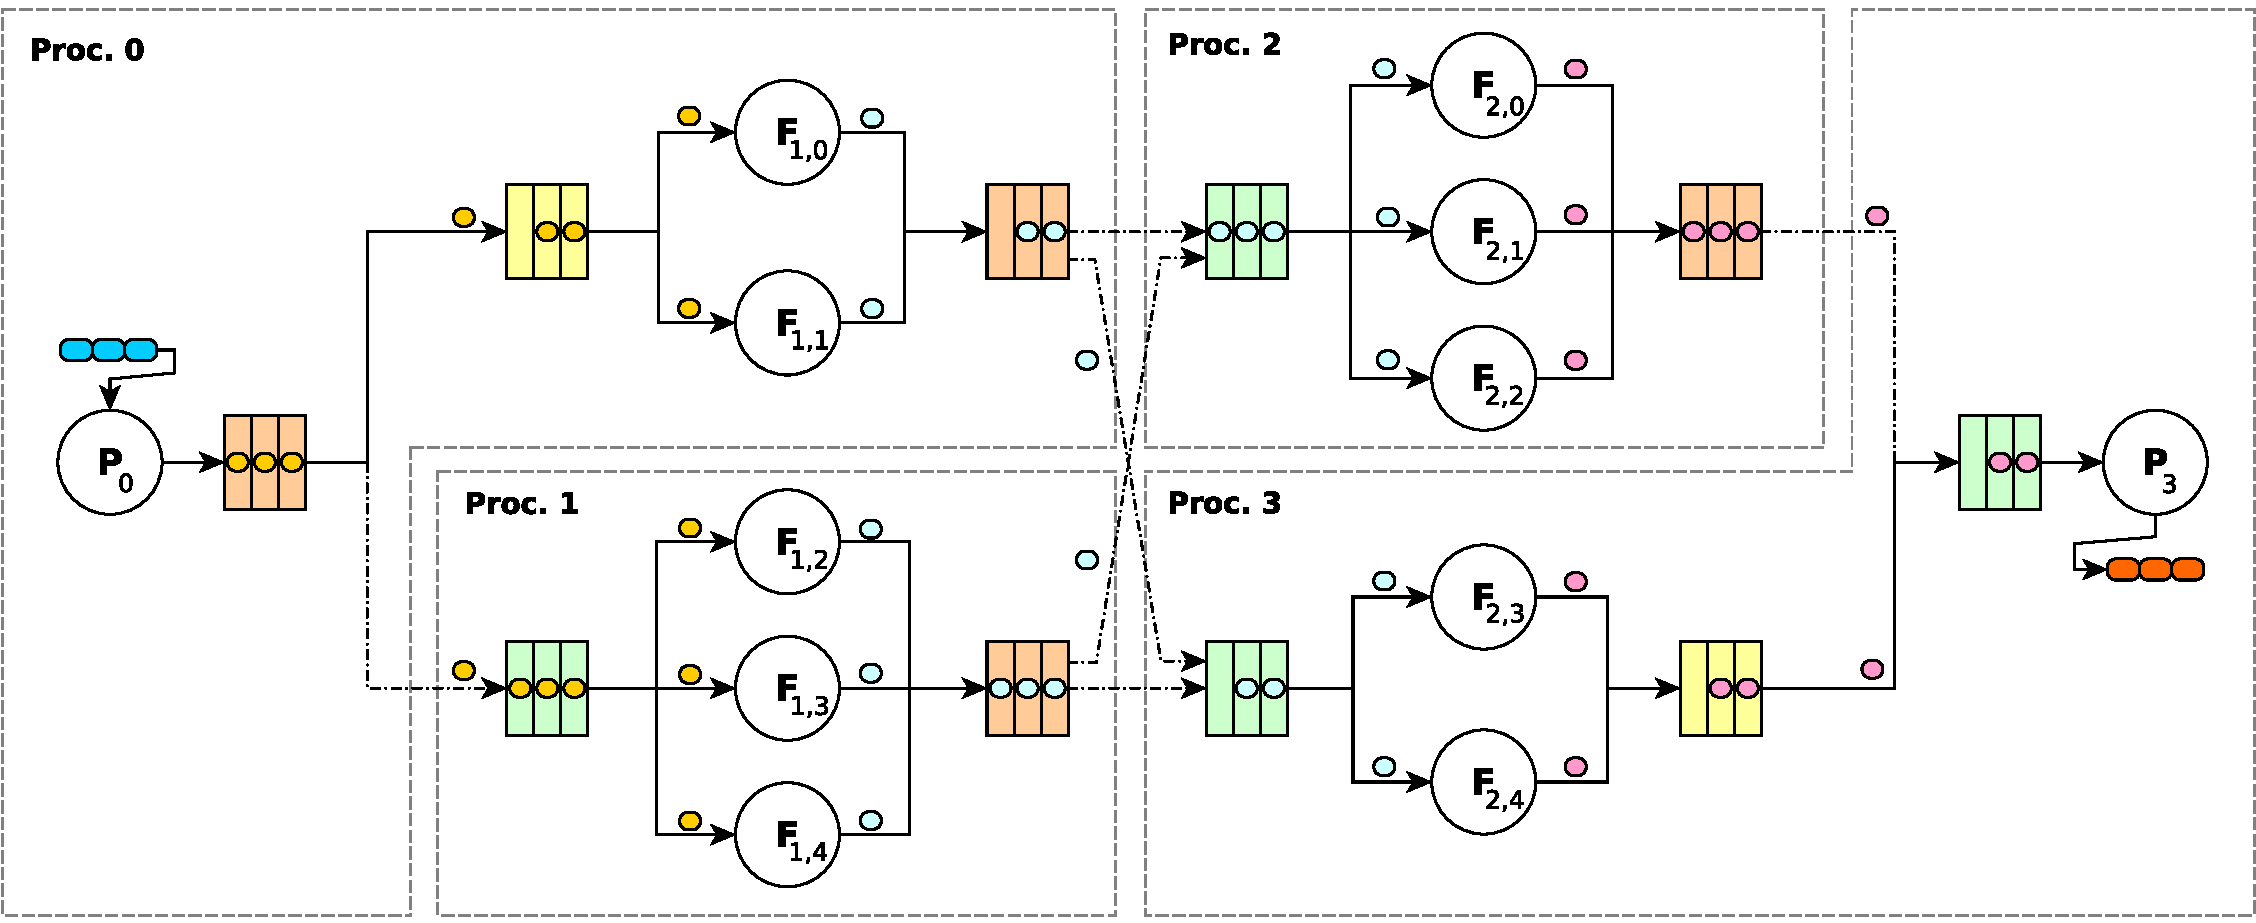
\includegraphics[width=0.95\textwidth]{figures/pipeline-mapping.pdf}\vspace{-0.2cm}
  \caption{Distribución de operadores de stream en procesos con $opp=3$.}\label{fig:mapping}
\end{figure*}
\vspace{0.35cm}

De acuerdo con esta fórmula, si el valor de $opp$ se establece de manera predeterminada, es decir, con Ec.~\ref{eq:opp}, todos los procesos ejecutan el mismo número de operadores excepto el último, que ejecuta todos los operadores restantes. De lo contrario, si $opp$ ha sido establecido por el usuario y es mayor que el establecido por defecto, entonces algunos últimos procesos podrían no ejecutar ningún operador. Tenga en cuenta también que el algoritmo de distribución selecciona operadores consecutivos para mapearlos en procesos \acrshort{mpi}, es decir, siguiendo el mismo orden en el que aparecen en el patrón de Pipeline.

La Figura~\ref{fig:mapping} representa una tubería de cuatro etapas compuesta por dos patrones de granja en la segunda y tercera etapas, que se ejecuta con 5 réplicas cada una. En este caso, la granularidad de agrupación o $opp$ se ha calculado de forma predeterminada utilizando Ec.~\ref{eq:opp}. Dado que cada proceso ejecuta los 3 operadores consecutivos correspondientes a los devueltos por Ec.~\ref{eq:range}. Por lo tanto, el mismo proceso de \acrshort{mpi} puede ejecutarse, utilizando la política de memoria compartida local, en etapas de Pipeline y/o réplicas de Farm. 

En general, esta política de ejecución de \acrshort{mpi} permite que los patrones \acrshort{grppi} se ejecuten en plataformas distribuidas de múltiples núcleos, aprovechando el paralelismo inter e intranodo. Además, gracias a su algoritmo de distribución de operadores, es capaz de distribuir automáticamente operadores siguiendo el orden lógico de transmisión.

%This policy allows the hybrid execution of those patterns when the number of total operators (\Pipeline stages and \Farm replicas) is higher than the number of \acrshort{mpi} processes. This is accomplished by collapsing contiguous \Pipeline operators or \Farm replicas onto multi-threaded processes.

% \begin{lstlisting}[linewidth=1\columnwidth,caption={SPSC queue of the \acrshort{mpi} back end.},label={lst:mpi-spsc-queue},frame=single]
% #include <boost/mpi.hpp>
% template <typename T>
% class mpi_spsc_queue {
%  private:
%   std::deque<mpi::request> buffer_;
%   int buffer_size_, rank_recv_;
%   bool pending_req_= false;
%   mpi::request req;
%   T item_;
%   ...
%  public:
%   ...
%   bool push (T item) {
%     // check for done requests
%     while (!buffer_.empty()) {
%       auto req = buffer_.front();
%       req.test() ? buffer_.pop_front() : break;
%     }
%     // send item async and store request
%     buffer_.push_back(comm_.isend(rank_recv_, tag_, item));
%   };
%   T pop() {
%     // request for the first element
%     if (!pending_req_) {
%       req = comm_.irecv(mpi::any_source, tag_, item_);
%       pending_req_ = true;
%     }
%     // wait for the previous item and request the next one
%     req.wait();
%     T item = item_;
%     req = comm_.irecv(mpi::any_source, tag_, item_);
%     return item;
%   };
% } 
% \end{lstlisting}

%\afterpage{\blankpage} % blank page

\lhead[\thepage]{CAPÍTULO \thechapter. EVALUACIÓN EXPERIMENTAL}
\chead[]{}
\rhead[Patrones de programación paralelos de alto nivel en arquitecturas de memoria distribuida\leftmark]{\thepage}
\renewcommand{\headrulewidth}{0.5pt}

\lfoot[]{}
\cfoot[]{}
\rfoot[]{}
\renewcommand{\footrulewidth}{0pt}

%% This is an example first chapter.  You should put chapter/appendix that you
%% write into a separate file, and add a line \include{yourfilename} to
%% main.tex, where `yourfilename.tex' is the name of the chapter/appendix file.
%% You can process specific files by typing their names in at the 
%% \files=
%% prompt when you run the file main.tex through LaTeX.
\chapter{Evaluación experimental}
\label{ch:evaluacion_experimental}
\markboth{}{EVALUACIÓN EXPERIMENTAL}

Este capítulo presenta la evaluación experimental de \acrshort{grppi} para plataformas de memoria distribuida. En primer lugar se describen los experimentos y la plataforma sobre la cual se han realizado (Sección \ref{sec:descripcion_experimentos}). Posteriormente se realiza un estudio de usabilidad (Sección \ref{sec:estudio_usabilidad}). Por último se realiza un análisis de rendimiento de la nueva implementación.

\section{Descripción de los experimentos}
\label{sec:descripcion_experimentos}

En esta sección, llevamos a cabo una evaluación experimental del back-end \acrshort{grppi} \acrshort{mpi} desde los puntos de vista de la usabilidad y el rendimiento. Para esta evaluación, empleamos los siguientes componentes de hardware y software:

\begin{itemize}

\item \textbf{Plataforma de destino}. La evaluación se ha llevado a cabo en un clúster homogéneo de ocho nodos, cada uno compuesto por un procesador Intel Xeon Broadwell E5-2603 v4 con 12 cores a 1.70\,GHz, 15\,MB de caché L3 y 128\,GB de \acrshort{ram} DDR3. El sistema operativo es Linux Ubuntu 16.04.3 LTS con el kernel 4.4.0-97. Los nodos están interconectados mediante un switch Ethernet de un Gigabit.

\item \textbf{Software}. Aprovechamos el nuevo back-end \acrshort{grppi} \acrshort{mpi} construido sobre \acrshort{grppi} v0.4~\cite{grppi-github}, junto con los respectivos back-end de memoria compartida y memoria distribuida, hilos de C ++11 y \acrshort{mpi}-3.1, implementados por \acrshort{mpi}CH v3.2.1. Tenga en cuenta que el back-end de \acrshort{mpi} se implementó con Boost \acrshort{mpi} v1.66.0. El compilador de C ++ utilizado para ensamblar \acrshort{grppi} fue GCC v7.2.0 que ya admite el estándar C ++ 14.

\item \textbf{Caso de uso}. Para evaluar los patrones distribuidos de Pipeline y Farm, aprovechamos una aplicación de transmisión que se encarga del cómputo de Mandelbrot, de forma que se crean imágenes para montar una animación de zoom fractal y aplicar el filtro de desenfoque gaussiano (Blur filter) en cada uno de los fotogramas generados. Concretamente, esta aplicación basada en Pipeline consta de las siguientes etapas:

\begin{description}
\item[Generador] devuelve valores de zoom crecientes monótonamente lineales, que se pasan a la etapa de Mandelbrot.
\item[Mandelbrot] toma el zoom recibido por el generador y calcula la trama de Mandelbrot correspondiente a dicho valor de zoom y las coordenadas del punto de interés.
\item[Gaussian blur] toma el frame calculado por la etapa anterior y aplica el filtro de desenfoque gaussiano a ellos, usando un kernel de 3$\times$3 píxels.
\item[Consumidor] guarda cada uno de los frames en el disco usando el formato BMP.
\end{description}

\end{itemize}

\vspace{0.35cm}
\begin{lstlisting}[linewidth=1\columnwidth,caption={Implementación Mandelbrot en Boost \acrshort{mpi}.},label=lst:mpimandelcode,frame=single]
int frame= 0;
int num_frames= 1000;
// Main Pipeline
grppi::Pipeline(mpi_exec,
  // Zoom generation
  [&]() -> std::experimental::optional<double> {
    if (frame++ == num_frames) return {};
      zoom-= zoom * 0.1;
    return zoom;
  },
  // Farm mandelbrot stage
  grppi::Farm(4,
    [&](auto zoom){
       return mandelbrot(height, width, poi_x, poi_y, zoom);
    }
  ),
  // Farm blur stage
  grppi::Farm(4,
    [&](auto image){
      return blur(height, width, kernel, image);
    }
  ), 
  // Consuming stage
  [&](auto image){
    save_bmp(height, width, image);
  }
);
\end{lstlisting}
\vspace{0.35cm}

Como se sabe generalmente, el conjunto de Mandelbrot es el conjunto de números complejos $c$ para los cuales la función $f_{c}(z)=z^{2}+c$ no diverge cuando se itera desde $z=0$, es decir, para el cual la secuencia $f_{c}(0)$, $f_{c}(f_{c}(0))$, etc., permanece limitada en valor absoluto. Por lo tanto, las imágenes de Mandelbrot pueden crearse muestreando los números complejos y determinando, para cada punto de muestra $c$, si el resultado de iterar la función anterior va al infinito. Luego, tratando las partes real e imaginaria de $c$ como coordenadas de imagen $(x+yi)$ en el plano complejo, los píxeles pueden colorearse de acuerdo con la rapidez con la secuencia $z_{n}^{2}+c$ diverge. Esta es la clave para comprender la naturaleza heterogénea de esta operación, donde la velocidad de divergencia en el punto de interés y el valor del zoom dictan el número de iteraciones para calcular un frame dado. Por el contrario, el operador de desenfoque gaussiano tiene una carga de trabajo casi homogénea para procesar cada uno de los frames. En nuestro caso de uso específico, el caso de uso de Mandelbrot se configuró para generar 1,000 frames y hasta 1,000 iteraciones para calcular cada frame del Mandelbrot.

\vspace{0.35cm}
\begin{lstlisting}[linewidth=1\columnwidth,caption={Implementación Mandelbrot en \acrshort{grppi} \acrshort{mpi}.},label=lst:grppimandelcode,frame=single]
std::vector<color> image;
if (world.rank() == 0) { // Zoom generator
  for(int frame= 0; frame < num_frames; frame++) {
    zoom-= zoom * 0.1;
    world.send(world.rank()+1, 0, zoom);
  }
}
else if (world.rank() == 1) { // Mandelbrot stage
  for(int frame= 0; frame < num_frames; frame++) {
    world.recv(world.rank()-1, 0, zoom);
    image = mandelbrot(height, width, poi_x, poi_y, zoom);
    world.send(world.rank()+1, 0, image);
  }
}
else if (world.rank() == 2) { // Blur stage
  for(int frame= 0; frame < num_frames; frame++) {
    world.recv(world.rank()-1, 0, image);
    image = blur(height, width, kernel, image);
    world.send(world.rank()+1, 0, image);
  }
} 
else if (world.rank() == 3) { // Consuming stage
  for(int frame= 0; frame < num_frames; frame++) {
    world.recv(world.rank()-1, 0, image);
    save_bmp(height, width, image);
  }
}
\end{lstlisting}
\vspace{0.35cm}

Dado el paralelismo natural de esta aplicación, donde cada uno de los fotogramas de animación se puede calcular de forma independiente, las etapas del Pipeline Mandelbrot y Gaussian blur pueden ser replicadas mediante el patrón Farm, por lo que pueden procesar fotogramas individuales. Por lo tanto, pueden surgir varias composiciones dependiendo de la paralelización de estas etapas, es decir, \texttt{(p|p|p|p)}, \texttt{(p|f|p|p)}, \texttt{(p|p|f|p)}, y \texttt{(p|f|f|p)}.

% As studied in Exercise~\ref{mandelbrot}, images of the Mandelbrot set exhibit an elaborate and infinitely complicated boundary that reveals progressively ever-finer recursive detail at increasing magnifications of the core function (remember the \texttt{zoom} variable). The ``style'' of this repeating detail depends on the region of the set being examined. The set's boundary also incorporates smaller versions of the main shape, so the fractal property of self-similarity applies to the entire set, and not just to its parts.

En las secciones siguientes, analizamos la usabilidad y el rendimiento de los patrones \acrshort{grppi} Pipeline y Farm distribuidos utilizando el punto de referencia mencionado anteriormente con diferentes configuraciones de grado de paralelismo con respecto al número de procesos \acrshort{mpi} y subprocesos de trabajo utilizados en las etapas de Farm. Además, evaluamos los costes del uso de \acrshort{grppi} con respecto a la paralelización directa de la aplicación a través de \acrshort{mpi}.

\section{Estudio de la usabilidad}
\label{sec:estudio_usabilidad}

Para analizar la usabilidad y la productividad de la interfaz de patrones propuesta y el nuevo back-end de \acrshort{mpi}, utilizamos la herramienta analizadora Lizard~\cite{lizard} para obtener dos métricas bien conocidas: Líneas de código (LOCs) y el Número de Complejidad Ciclomática de McCabe's (CCN)~\cite{McCabe:1976}. Básicamente, utilizamos estas métricas para analizar las diferentes versiones de casos de uso, es decir, con y sin utilizar la interfaz \acrshort{grppi}. La Tabla~\ref{tab:lines} resume el porcentaje de LOCs adicionales introducidos en el código fuente secuencial para implementar las versiones paralelas usando \acrshort{mpi} y la interfaz \acrshort{grppi}, junto con sus CCNs correspondientes. Como se observa, la implementación de composiciones más complejas a través de \acrshort{mpi} conduce a códigos fuente más grandes y más complejos, mientras que para \acrshort{grppi} el número de LOCs radicionales permanece constante. Esta diferencia se debe principalmente a las colas de comunicación requeridas para implementar el patrón Farm. Centrándonos en \acrshort{grppi}, observamos que el esfuerzo de paralelización es casi insignificante: incluso la composición más compleja aumenta casi el 4.2\,\% de LOCs. Además, al cambiar a \acrshort{grppi} para que use una política de ejecución particular, solo se necesita cambiar un único argumento en la llamada a la función de patrón. Con respecto a la complejidad ciclomática para \acrshort{mpi}, observamos que sus CCNs son aproximadamente proporcionales al aumento del porcentaje de LOCs. . Por el contrario, la interfaz \acrshort{grppi} tiene CCN constantes para todas las composiciones de Pipeline.

\vspace{0.35cm}
\newcolumntype{C}{>{\centering\let\newline\\\arraybackslash\hspace{0pt}}p{1.2cm}}
\begin{table}[ht!]
\centering
%\vspace{-0.8cm}
\caption{Porcentaje de LOCs adicionales con respecto a la versión secuencial y los CNNs para las composiciones de Pipeline.}\label{tab:lines}\vspace{-0.15cm}
\small
\scalebox{1}{
\begin{tabular}{|c|C|C|C|C|}\hline
%  Pipeline  & \multicolumn{2}{c|}{\textbf{MPI}}  & \multicolumn{2}{c|}{\textbf{\acrshort{grppi}}}\\\cline{2-5}
% composición & LOCs & CCNs & LOCs & CCNs \\\hline\hline
% \texttt{(p|p|p|p)}  & $+$75.1\,\%  & 18  & $+$4.2\,\%   & 7  \\
% \texttt{(p|f|p|p)}  & $+$130.4\,\% & 38  & $+$4.2\,\%   & 7  \\
% \texttt{(p|p|f|p)}  & $+$130.4\,\% & 38  & $+$4.2\,\%   & 7  \\
% \texttt{(p|f|f|p)}  & $+$185.8\,\% & 58  & $+$4.2\,\%   & 7  \\\hline

 Composición  & \multicolumn{2}{c|}{\textbf{\% LOCs adicionales}}  & \multicolumn{2}{c|}{\textbf{CCN}} \\\cline{2-5}
Pipeline & \acrshort{mpi} & \acrshort{grppi} & \acrshort{mpi} & \acrshort{grppi} \\\hline\hline
\texttt{(p|p|p|p)}  & $+$10.3\,\%  & $+$4.2\,\% & 9 & 7  \\
\texttt{(p|f|p|p)}  & $+$130.4\,\% & $+$4.2\,\% & 38 & 7  \\
\texttt{(p|p|f|p)}  & $+$130.4\,\% & $+$4.2\,\% & 38 & 7  \\
\texttt{(p|f|f|p)}  & $+$185.8\,\% & $+$4.2\,\% & 58 & 7  \\\hline
\end{tabular}}
%\vspace{-0.7cm}
\end{table}
\vspace{0.35cm}

Finalmente, realizamos una comparación lado a lado entre las interfaces Boost \acrshort{mpi} y \acrshort{grppi} implementando una versión simplificada del caso de uso de Mandelbrot. % As can be seen in Listing~\ref{lst:grppimandelcode}, the \grppi code follows a comprehensible and readable structure, which clearly shows the compositions among stream operators. On the contrary, the \acrshort{mpi} code, shown in Listing~\ref{lst:mpimandelcode}, is not as structured and easy to read as the \grppi implementation.\footnote{For the sake of simplicity, we have replaced the use of queues by synchronous communications, so no computations overlap communications in this case.} 
Como se puede ver en el Listado \ref{lst:mpimandelcode}, la implementación de \acrshort{mpi} distingue claramente las instrucciones y comunicaciones que deben ser ejecutadas por cada uno de los procesos. \footnote{Para mayor simplicidad, hemos reemplazado el uso de colas por comunicaciones síncronas, por lo que no hay cálculos que se superpongan a las comunicaciones en este caso.}. Por otro lado, el código \acrshort{grppi}, que se muestra en el Listado~\ref{lst:grppimandelcode}, se centra más en la estructura del algoritmo de la aplicación que en las comunicaciones entre procesos.
%follows a comprehensible and readable structure, which clearly shows the application algorithm structure. 
%is more structured and easier to read than the \acrshort{mpi} implementation.
%Thus, to properly understand the application behavior, users need to carefully analyze its structure along with the execution flow to known which portions of the code will be executed by each of the processes.
En pocas palabras, aunque ambas interfaces proporcionan interfaces de alto nivel, concluimos que las implementaciones de patrones ofrecidas por \acrshort{grppi} ayudan a mejorar tanto la productividad como la capacidad de mantenimiento.

\section{Análisis de rendimiento}
\label{sec:analisis_rendimiento}

En esta sección, evaluamos el rendimiento y la escalabilidad de la aplicación Mandelbrot implementada con la interfaz \acrshort{grppi} utilizando la política \acrshort{mpi} junto con el back-end de memoria compartida basado en hilos C ++ 11. Evaluamos el rendimiento de la aplicación utilizando solo el back-end de memoria compartida. Además, hemos limitado la cantidad de núcleos por nodo para simular diferentes escenarios de clúster. Tenga en cuenta que solo nos centramos en la composición del Pipeline \texttt{(p|f|f|p)}, ya que ofrece el mejor rendimiento y puede escalarse mejor entre los nodos del clúster.

La Figura~\ref{fig:mandel-pffp} representa la escala de speedup cuando se usa de 1 a 8 nodos de clúster y se ejecuta de 1 a 12 subprocesos por nodo para resoluciones de cuadros cuadrados de 200, 400 y 800 píxeles con respecto a la aplicación secuencial. Es importante destacar que cada experimento ejecuta tantos operadores (etapas de Pipeline y réplicas de Farm) como la cantidad total de subprocesos ejecutados en los nodos. Como se observa, el speedup logrado por \acrshort{mpi} usando un solo nodo es igual a la memoria compartida; esto viene dado por el hecho de que el back-end \acrshort{mpi} delega completamente en el back-end de la memoria compartida cuando se ejecuta en un nodo. En este primer intento del experimento, establecemos el mismo número de réplicas de Farm en las etapas de Mandelbrot y de Gaussian Blur. Como puede verse, para 1, 2 y 4 nodos, la aplicación escala linealmente con el número de subprocesos por nodo, con una eficiencia sostenida de aproximadamente 45\,\%. Sin embargo, para 8 nodos, el rendimiento se degrada desde 6 subprocesos por nodo, ya que la etapa de Mandelbrot causa un importante cuello de botella en la interconexión debido a los niveles de producción desequilibrados. La eficiencia máxima, en este caso, es 26\,\%. Esto se debe a que la carga de trabajo de Mandelbrot por cada frame es mucho mayor que la aplicación del operador Gaussian Blur.

Para lidiar con este desequilibrio, hemos calculado empíricamente la relación entre los rendimientos de las etapas Mandelbrot y Blur, que nos sirvió para determinar el número óptimo de réplicas en las etapas correspondientes de Farm. Básicamente, hemos calculado esta relación usando promedios de rendimiento de ambas etapas para las diferentes resoluciones de frame. Usando esta proporción, asignamos 1 réplica de Blur por cada 25 réplicas de Mandelbrot. Sin embargo, esta relación no ofrece rendimientos ideales dada la naturaleza heterogénea de la carga de trabajo del conjunto de Mandelbrot. La Figura~\ref{fig:mandel-pfsp} muestra el rendimiento logrado para la diferente cantidad de nodos y subprocesos por experimentos de nodo y el uso de la relación antes mencionada. Como se observa, de 1 a 4 nodos, la eficiencia mejora significativamente con respecto al experimento anterior, de 45\,\% a 68\,\%. Los resultados también revelan escalas de rendimiento relativamente buenas para todos los tamaños de frame.  Por otro lado, para 8 nodos, la aplicación muestra un peor rendimiento cuando se utilizan más de 6 subprocesos por núcleo. Esta degradación se debe principalmente a la diferencia entre la carga de trabajo de la etapa y los gastos generales de comunicación inherentes. Por esta razón, para tamaños de cuadros grandes, el rendimiento alcanzado es ligeramente mejor, ya que los cálculos paralelos pagan los tiempos de serialización y transferencia de datos requeridos. En cualquier caso, para 8 nodos, la eficiencia obtenida usando etapas de Farm equilibradas aumenta de 26\,\% a 45\,\%.

\vspace{0.35cm}
\begin{figure}[!tbp]
\centering
\begin{subfigure}[b]{0.32\textwidth}
  \centering
  \includegraphics[width=0.95\linewidth]{figures/graph-mpi-200-pffp.pdf}
  \caption{Resolución de imagen 200$\times$200.}
  \label{fig:mandel-pffp-200}
\end{subfigure}%
\hfill
\begin{subfigure}[b]{0.32\textwidth}
  \centering
  \includegraphics[width=0.95\linewidth]{figures/graph-mpi-400-pffp.pdf}
  \caption{Resolución de imagen 400$\times$400.}
  \label{fig:mandel-pffp-400}
\end{subfigure}
\hfill
\begin{subfigure}[b]{0.32\textwidth}
  \centering
  \includegraphics[width=0.95\linewidth]{figures/graph-mpi-800-pffp.pdf}
  \caption{Resolución de imagen 800$\times$800.}
  \label{fig:mandel-pffp-800}
\end{subfigure}
\caption{Caso de uso de Mandelbrot con Pipeline \texttt{(p|f|f|p)} con mismo número de réplicas de Farm.}
\label{fig:mandel-pffp}
\end{figure}
\vspace{0.35cm}

A partir de estos experimentos, podemos concluir que la interfaz \acrshort{grppi} propuesta puede ayudar a implementar aplicaciones científicas de flujo distribuido a expensas de gastos indirectos insignificantes. En un experimento separado, evaluamos la sobrecarga introducida por \acrshort{grppi} con respecto a utilizar \acrshort{mpi} directamente. Esta sobrecarga fue menor a 0.1\,\%.

\vspace{0.35cm}
\begin{figure}[!tbp]
\centering
\begin{subfigure}[b]{0.32\textwidth}
  \centering
  \includegraphics[width=0.95\linewidth]{figures/graph-mpi-200-pfsp.pdf}
  \caption{Resolución de imagen 200$\times$200.}
  \label{fig:mandel-pfsp-200}
\end{subfigure}%
\hfill
\begin{subfigure}[b]{0.32\textwidth}
  \centering
  \includegraphics[width=0.95\linewidth]{figures/graph-mpi-400-pfsp.pdf}
  \caption{Resolución de imagen 400$\times$400.}
  \label{fig:mandel-pfsp-400}
\end{subfigure}
\hfill
\begin{subfigure}[b]{0.32\textwidth}
  \centering
  \includegraphics[width=0.95\linewidth]{figures/graph-mpi-800-pfsp.pdf}
  \caption{Resolución de imagen 800$\times$800.}
  \label{fig:mandel-pfsp-800}
\end{subfigure}
\caption{Caso de uso de Mandelbrot con Pipeline \texttt{(p|f|f|p)} con un número ajustado de réplicas de Farm.}
\label{fig:mandel-pfsp}
\end{figure}
\vspace{0.35cm}

%\afterpage{\blankpage} % blank page
\lhead[\thepage]{CAPÍTULO \thechapter. PLANIFICACIÓN DEL PROYECTO}
\chead[]{}
\rhead[Patrones de programación paralelos de alto nivel en arquitecturas de memoria distribuida\leftmark]{\thepage}
\renewcommand{\headrulewidth}{0.5pt}

\lfoot[]{}
\cfoot[]{}
\rfoot[]{}
\renewcommand{\footrulewidth}{0pt}

%% This is an example first chapter.  You should put chapter/appendix that you
%% write into a separate file, and add a line \include{yourfilename} to
%% main.tex, where `yourfilename.tex' is the name of the chapter/appendix file.
%% You can process specific files by typing their names in at the 
%% \files=
%% prompt when you run the file main.tex through LaTeX.
\chapter{Planificación del proyecto}
\label{ch:planificacion_proyecto}
\markboth{}{PLANIFICACION DEL PROYECTO}

Este capítulo presenta una planificación detallada del proyecto. Este proyecto ha sido realizado en colaboración con el grupo de investigación \acrshort{arcos} de la Universidad Carlos III de Madrid durante la realización del Máster en Ciencia y Tecnología Informática de la misma universidad. El proyecto comenzó el 8 de enero de 2018 y finalizó el 5 de septiembre de 2018, con un total de 9 meses de trabajo.

Dado que este proyecto de investigación incluye una parte de desarrollo, ambos lados, la investigación y el desarrollo tuvieron que fusionarse para obtener una metodología de investigación y planificación adecuadas. La metodología aplicada se muestra en la Figura\ref{fig:methodology}.

\vspace{0.35cm}
\begin{figure}[htbp]
 	\centering
 	\includegraphics[width=0.75\textwidth]{figures/methodology.pdf}
 	\caption{Metodología de investigación empleada.}
	\label{fig:methodology}
\end{figure}
\vspace{0.35cm}

Donde:

\begin{itemize}

\item \textbf{Identificación del problema} que estamos tratando de resolver.

\item \textbf{Definición de los objetivos} del proyecto.

\item \textbf{Estado de la cuestión a investigar}: sintetiza el más alto nivel del campo científico.

\item \textbf{Propuesta de solución}: diseño y definición de la solución.

\item \textbf{Proceso de desarrollo}: de la solución propuesta.

\item \textbf{Evaluación de la solución}: analizar diferentes casos de estudio.

\item \textbf{Resultados de investigación y publicación}: publica los resultados de la tesis de máster en varias revistas y conferencias.

\item \textbf{Documentación de la tesis}: escribe el informe final.

\end{itemize}

El diagrama de Gantt (Figura \ref{fig:gantt}) muestra todas las tareas realizadas durante el desarrrollo de este trabajo.

\vspace{0.5cm}
\begin{figure}[htbp]
 	\centering
 	\includegraphics[width=16.5cm]{figures/DiagramaJavi.pdf}
 	\caption{Diagrama de Gantt.}
	\label{fig:gantt}
\end{figure}
\vspace{0.35cm}

%\afterpage{\blankpage} % blank page


\lhead[\thepage]{CAPÍTULO \thechapter. CONCLUSIONES Y TRABAJO FUTURO}
\chead[]{}
\rhead[Patrones de programación paralelos de alto nivel en arquitecturas de memoria distribuida\leftmark]{\thepage}
\renewcommand{\headrulewidth}{0.5pt}

\lfoot[]{}
\cfoot[]{}
\rfoot[]{}
\renewcommand{\footrulewidth}{0pt}

%% This is an example first chapter.  You should put chapter/appendix that you
%% write into a separate file, and add a line \include{yourfilename} to
%% main.tex, where `yourfilename.tex' is the name of the chapter/appendix file.
%% You can process specific files by typing their names in at the 
%% \files=
%% prompt when you run the file main.tex through LaTeX.
\chapter{Conclusiones y trabajo futuro}
\label{ch:conclusiones_trabajo_futuro}
\markboth{}{CONCLUSIONES Y TRABAJO FUTURO}

Este capítulo presenta las conclusiones de este proyecto y el trabajo futuro. En primer lugar se exponen las conclusiones y los resultados obtenidos (Sección \ref{sec:conclusiones}). Por último se expone el trabajo futuro a realizar en esta línea de investigación.

\section{Conclusiones}
\label{sec:conclusiones}

En este trabajo, hemos ampliado \acrshort{grppi}, una interfaz de patrones paralelos genérica y reutilizable, con un nuevo back-end \acrshort{mpi}, que permite la ejecución de los patrones Pipeline y Farm en plataformas distribuidas. Para admitir escenarios híbridos, el back-end también combina una política de ejecución de memoria compartida intranodo que, si es necesario, se utiliza para ejecutar múltiples operadores de Pipeline y/o operadores de Farm dentro del mismo proceso \acrshort{mpi}. En general, el diseño compacto de \acrshort{grppi} facilita el desarrollo de aplicaciones de transmisión de datos, mejorando la flexibilidad y la portabilidad, a la vez que explota el paralelismo inter e intranodo.

Como se demostró a lo largo de la evaluación experimental, el caso de uso de Mandelbrot, implementado con patrones de Pipeline y Farm distribuidos, logra ganancias de speedup considerables en comparación con la versión secuencial correspondiente. En cualquier caso, siempre es importante equilibrar las etapas de Pipeline de acuerdo con las cargas de trabajo de la etapa. También demostramos que el aprovechamiento de \acrshort{grppi} reduce considerablemente el número de LOCs y la complejidad ciclomática con respecto a la implementación utilizando directamente \acrshort{mpi}. Además, gracias a la comparación cualitativa de las dos interfaces de alto nivel, \acrshort{grppi} y \acrshort{mpi}, concluimos que \acrshort{grppi} conduce a códigos más estructurados y legibles, y por lo tanto, mejora su mantenibilidad general. En general, la implementación de un back-end distribuido mediante \acrshort{mpi} se ha motivado principalmente por las necesidades de escalamiento y el desarrollo de nuevos modelos de programación para aplicaciones científicas \acrshort{dasp}.  Además, nuestro interés con este back-end proviene de la amplia adopción de \acrshort{mpi} en las supercomputadoras de hoy, que actualmente no tiene soporte estándar para el procesamiento de streaming~\cite{peng2017}. Por estas razones, creemos que el back-end presentado puede ser de gran ayuda en el desarrollo de aplicaciones de streaming en C ++.

Por lo tanto, podemos concluir que se han logrado los objetivos citados en comienzo del documento:

\begin {itemize}
\item \textbf{O1}: Hemos presentado una nueva política de ejecución de \acrshort{grppi}-MPI para entornos distribuidos e híbridos para los patrones paralelos \emph{Pipeline} y \emph{Farm}.
\item \textbf{O2}: Se ha descrito el diseño de la interfaz \acrshort{grppi} y las políticas internas de \acrshort{mpi} para permitir la ejecución distribuida e híbrida de aplicaciones \acrshort{dasp}.
\item \textbf{O3}: Se ha presentado un nuevo operador para patrones de \emph{streaming} que, como un contenedor, permite a los usuarios reemplazar la política de ejecución predeterminada de un patrón.
\item \textbf{O4}: Hemos analizado la usabilidad del patrón en términos de líneas de código y complejidad ciclomática, y realizando una comparación \emph{side-by-side} de ambas interfaces de programación \acrshort{grppi} y \acrshort{mpi}.
\item \textbf{O5}: Se han evaluado los patrones distribuidos \emph{Pipeline} y \emph{Farm} de \emph{streaming} desde los puntos de vista de usabilidad y rendimiento usando una aplicación que renderiza frames de Mandelbrot bajo diferentes configuraciones híbridas.
\end {itemize}

Además, este trabajo ha dado como resultado una publicación en la conferencia internacional EuroMPI 2018 que se celebrará en Septiembre en Barcelona (España).

\begin{itemize}
\item \textbf{Supporting \acrshort{mpi}-Distributed Stream Parallel Patterns in \acrshort{grppi}}\cite{eurompi2018}. \textit{Javier Fernández Muñoz, Manuel F. Dolz, David del Rio Astorga, Javier Prieto Cepeda and J. Daniel García}, EuroMPI 2018, Barcelona.
\end{itemize}

\section{Trabajo futuro}
\label{sec:trabajo_futuro}

Como trabajo futuro, planeamos admitir nuevos algoritmos para la distribución de operadores en procesos e introducir un nuevo operador para permitir a los usuarios reemplazar la política de ejecución predeterminada de un operador concreto en una etapa de Pipeline. También planeamos implementar otros patrones de streaming, como filter o Stream-Reduce, dentro de la política de ejecución de \acrshort{mpi} y mejorar las colas de comunicación para usar comunicaciones \acrshort{mpi} de un solo lado.

\afterpage{\blankpage} % blank page

%\include{appendixa}

%\printglossary[type=\acronymtype,title=Abbreviations]
%\printglossary

%Some text between the list of acronyms and the glossary.

%\printglossary
%\addcontentsline{toc}{chapter}{Glossary}

%\printglossary
%\addcontentsline{toc}{chapter}{Glosario}

\printglossary[type=\acronymtype,title={Acrónimos}]
\addcontentsline{toc}{chapter}{Acrónimos}


%\printglossary[type=\acronymtype]
%\addcontentsline{toc}{chapter}{Acronyms}

\afterpage{\blankpage} % blank page

\cleardoublepage
\phantomsection
\lhead[\thepage]{BIBLIOGRAFÍA}
\chead[]{}
\rhead[Patrones de programación paralelos de alto nivel en arquitecturas de memoria distribuida]{\thepage}
\renewcommand{\headrulewidth}{0.5pt}

\lfoot[]{}
\cfoot[]{}
\rfoot[]{}
\renewcommand{\footrulewidth}{0pt}

%% This defines the bibliography file (main.bib) and the bibliography style.
%% If you want to create a bibliography file by hand, change the contents of
%% this file to a `thebibliography' environment.  For more information 
%% see section 4.3 of the LaTeX manual.
\begin{singlespace}
\addcontentsline{toc}{chapter}{Bibliografía}
\bibliography{bib/bib}
\bibliographystyle{ieeetr}
\end{singlespace}


\afterpage{\blankpage} % blank page
\clearpage

\end{document}